\documentclass[12pt,]{article}
\usepackage{lmodern}
\usepackage{amssymb,amsmath}
\usepackage{ifxetex,ifluatex}
\usepackage{fixltx2e} % provides \textsubscript
\ifnum 0\ifxetex 1\fi\ifluatex 1\fi=0 % if pdftex
  \usepackage[T1]{fontenc}
  \usepackage[utf8]{inputenc}
\else % if luatex or xelatex
  \ifxetex
    \usepackage{mathspec}
  \else
    \usepackage{fontspec}
  \fi
  \defaultfontfeatures{Ligatures=TeX,Scale=MatchLowercase}
    \setmainfont[]{Times New Roman}
\fi
% use upquote if available, for straight quotes in verbatim environments
\IfFileExists{upquote.sty}{\usepackage{upquote}}{}
% use microtype if available
\IfFileExists{microtype.sty}{%
\usepackage[]{microtype}
\UseMicrotypeSet[protrusion]{basicmath} % disable protrusion for tt fonts
}{}
\PassOptionsToPackage{hyphens}{url} % url is loaded by hyperref
\usepackage[unicode=true]{hyperref}
\hypersetup{
            pdftitle={Analysis of Factors Affecting Cover Crop Adoption on Almond Orchards in California},
            pdfauthor={Emily McNamara},
            pdfborder={0 0 0},
            breaklinks=true}
\urlstyle{same}  % don't use monospace font for urls
\usepackage[margin=2.0cm]{geometry}
\usepackage{color}
\usepackage{fancyvrb}
\newcommand{\VerbBar}{|}
\newcommand{\VERB}{\Verb[commandchars=\\\{\}]}
\DefineVerbatimEnvironment{Highlighting}{Verbatim}{commandchars=\\\{\}}
% Add ',fontsize=\small' for more characters per line
\usepackage{framed}
\definecolor{shadecolor}{RGB}{248,248,248}
\newenvironment{Shaded}{\begin{snugshade}}{\end{snugshade}}
\newcommand{\KeywordTok}[1]{\textcolor[rgb]{0.13,0.29,0.53}{\textbf{#1}}}
\newcommand{\DataTypeTok}[1]{\textcolor[rgb]{0.13,0.29,0.53}{#1}}
\newcommand{\DecValTok}[1]{\textcolor[rgb]{0.00,0.00,0.81}{#1}}
\newcommand{\BaseNTok}[1]{\textcolor[rgb]{0.00,0.00,0.81}{#1}}
\newcommand{\FloatTok}[1]{\textcolor[rgb]{0.00,0.00,0.81}{#1}}
\newcommand{\ConstantTok}[1]{\textcolor[rgb]{0.00,0.00,0.00}{#1}}
\newcommand{\CharTok}[1]{\textcolor[rgb]{0.31,0.60,0.02}{#1}}
\newcommand{\SpecialCharTok}[1]{\textcolor[rgb]{0.00,0.00,0.00}{#1}}
\newcommand{\StringTok}[1]{\textcolor[rgb]{0.31,0.60,0.02}{#1}}
\newcommand{\VerbatimStringTok}[1]{\textcolor[rgb]{0.31,0.60,0.02}{#1}}
\newcommand{\SpecialStringTok}[1]{\textcolor[rgb]{0.31,0.60,0.02}{#1}}
\newcommand{\ImportTok}[1]{#1}
\newcommand{\CommentTok}[1]{\textcolor[rgb]{0.56,0.35,0.01}{\textit{#1}}}
\newcommand{\DocumentationTok}[1]{\textcolor[rgb]{0.56,0.35,0.01}{\textbf{\textit{#1}}}}
\newcommand{\AnnotationTok}[1]{\textcolor[rgb]{0.56,0.35,0.01}{\textbf{\textit{#1}}}}
\newcommand{\CommentVarTok}[1]{\textcolor[rgb]{0.56,0.35,0.01}{\textbf{\textit{#1}}}}
\newcommand{\OtherTok}[1]{\textcolor[rgb]{0.56,0.35,0.01}{#1}}
\newcommand{\FunctionTok}[1]{\textcolor[rgb]{0.00,0.00,0.00}{#1}}
\newcommand{\VariableTok}[1]{\textcolor[rgb]{0.00,0.00,0.00}{#1}}
\newcommand{\ControlFlowTok}[1]{\textcolor[rgb]{0.13,0.29,0.53}{\textbf{#1}}}
\newcommand{\OperatorTok}[1]{\textcolor[rgb]{0.81,0.36,0.00}{\textbf{#1}}}
\newcommand{\BuiltInTok}[1]{#1}
\newcommand{\ExtensionTok}[1]{#1}
\newcommand{\PreprocessorTok}[1]{\textcolor[rgb]{0.56,0.35,0.01}{\textit{#1}}}
\newcommand{\AttributeTok}[1]{\textcolor[rgb]{0.77,0.63,0.00}{#1}}
\newcommand{\RegionMarkerTok}[1]{#1}
\newcommand{\InformationTok}[1]{\textcolor[rgb]{0.56,0.35,0.01}{\textbf{\textit{#1}}}}
\newcommand{\WarningTok}[1]{\textcolor[rgb]{0.56,0.35,0.01}{\textbf{\textit{#1}}}}
\newcommand{\AlertTok}[1]{\textcolor[rgb]{0.94,0.16,0.16}{#1}}
\newcommand{\ErrorTok}[1]{\textcolor[rgb]{0.64,0.00,0.00}{\textbf{#1}}}
\newcommand{\NormalTok}[1]{#1}
\usepackage{graphicx,grffile}
\makeatletter
\def\maxwidth{\ifdim\Gin@nat@width>\linewidth\linewidth\else\Gin@nat@width\fi}
\def\maxheight{\ifdim\Gin@nat@height>\textheight\textheight\else\Gin@nat@height\fi}
\makeatother
% Scale images if necessary, so that they will not overflow the page
% margins by default, and it is still possible to overwrite the defaults
% using explicit options in \includegraphics[width, height, ...]{}
\setkeys{Gin}{width=\maxwidth,height=\maxheight,keepaspectratio}
\IfFileExists{parskip.sty}{%
\usepackage{parskip}
}{% else
\setlength{\parindent}{0pt}
\setlength{\parskip}{6pt plus 2pt minus 1pt}
}
\setlength{\emergencystretch}{3em}  % prevent overfull lines
\providecommand{\tightlist}{%
  \setlength{\itemsep}{0pt}\setlength{\parskip}{0pt}}
\setcounter{secnumdepth}{5}
% Redefines (sub)paragraphs to behave more like sections
\ifx\paragraph\undefined\else
\let\oldparagraph\paragraph
\renewcommand{\paragraph}[1]{\oldparagraph{#1}\mbox{}}
\fi
\ifx\subparagraph\undefined\else
\let\oldsubparagraph\subparagraph
\renewcommand{\subparagraph}[1]{\oldsubparagraph{#1}\mbox{}}
\fi

% set default figure placement to htbp
\makeatletter
\def\fps@figure{htbp}
\makeatother

\usepackage{placeins}
\usepackage{etoolbox}
\makeatletter
\providecommand{\subtitle}[1]{% add subtitle to \maketitle
  \apptocmd{\@title}{\par {\large #1 \par}}{}{}
}
\makeatother
\usepackage{booktabs}
\usepackage{longtable}
\usepackage{array}
\usepackage{multirow}
\usepackage{wrapfig}
\usepackage{float}
\usepackage{colortbl}
\usepackage{pdflscape}
\usepackage{tabu}
\usepackage{threeparttable}
\usepackage{threeparttablex}
\usepackage[normalem]{ulem}
\usepackage{makecell}
\usepackage{xcolor}
\usepackage{caption}
\usepackage{graphicx}
\usepackage{siunitx}
\usepackage{hhline}
\usepackage{calc}
\usepackage{tabularx}

\title{Analysis of Factors Affecting Cover Crop Adoption on Almond Orchards in
California}
\providecommand{\subtitle}[1]{}
\subtitle{\url{https://github.com/emac2020/Almond-Survey-2020}}
\author{Emily McNamara}
\date{}

\begin{document}
\maketitle

\newpage

\tableofcontents  \newpage
\listoftables  \newpage
\listoffigures  \newpage

\section{Rationale and Research
Questions}\label{rationale-and-research-questions}

California is the epicenter of global almond production, producing 80\%
of the world's almond supply. As the forecasted growth of consumer
demand shows few signs of subsiding, farmers in California are
converting farmland to almond orchards at a considerable rate - from
428,000 acres in 1996 to 1,170,000 acres in 2019. However, the industry
is in a precarious position as almonds require 100\% pollination form
managed honey bees - a species that has witnessed significant decline in
population since 2006. The decline in managed honey bees is attributed
to poor nutrition, lack of diverse forage, stress from transporation,
and pesticide toxicity.

To mitigate the decline in managed honey bees and protect honey bee
health on almond orachards, experts determined several bee-friendly
practices that growers can adopt on their farms. One of these practices
is planting temporary forage called `cover crop' between tree rows to
increase the diversity and abundance of nutrient and pollen sources for
the honey bees.

This study uses data from a survey administered to almond producers and
farm managers throughout California to identify potential barriers in
adopting cover crop and understand why the practice of planting cover
crops is not widely adopted by almond producers.

To meet the research objectives, the primary research questions are:

\begin{itemize}
\tightlist
\item
  Where are the respondents' almond orchards located?
\item
  Which demographic factors affect whether or not respondents have
  planted cover crop in the last 5 years?
\item
  How does region affect whether or not the respondents have planted
  cover crop in the last 5 years?
\item
  How does respondent role in the almond operation affect whether or not
  the respondents have planted cover crop in the last 5 years?
\item
  How does respondent age affect whether or not the respondents have
  planted cover crop in the last 5 years?
\item
  How does the size of the almond operation affect whether or not the
  respondents have planted cover crop in the last 5 years?
\end{itemize}

\newpage

\section{Dataset Information}\label{dataset-information}

For the analysis, the following datasets were used:

\subsection{Almond Survey Results
Dataset}\label{almond-survey-results-dataset}

This dataset contains data of 301 completed responses from a survey that
was distributed to almond producers and farm managers throughout
California. The survey was launched on December 10th, 2019 and was
closed on February 5th, 2020. Data were collected using Qualtrics.

The downloaded file was saved in the project folder path
./Data/Raw/Almond\_Survey\_Results\_raw.csv on 2020-04-02

\subsubsection{Data Content Information}\label{data-content-information}

The dataset contains 24 columns. See the report's README for Almond
Survey Results Dataset: Column Names and Descriptions.

\subsection{Almond Survey Numeric Results
Dataset}\label{almond-survey-numeric-results-dataset}

This dataset contains the same responses as the Almond Survey Results
Dataset in section 2.1., but the dataset was downloaded from Qualtrics
in numerical answer form with split-answer columns.

The downloaded file was saved in the project folder path
./Data/Raw/Almond\_Survey\_Numeric\_Answers\_Raw.csv on 2020-04-02

\subsubsection{Data Content
Information}\label{data-content-information-1}

\paragraph{Table 1: Almond Survey Numeric Response Dataset Content
Information}\label{table-1-almond-survey-numeric-response-dataset-content-information}

The dataset contains 48 columns. See the report's README for Almond
Survey Numeric Response Dataset: Column Names and Descriptions.

\subsection{Naming Conventions and File
Formats}\label{naming-conventions-and-file-formats}

The files are named according to the following convention: Files are
named according to the following naming convention:
\texttt{databasename\_datatype\_details\_stage.format}, where:

\textbf{databasename} refers to the database from where the data
originated

\textbf{datatype} is a description of data

\textbf{details} are additional descriptive details, particularly
important for processed data

\textbf{stage}refers to the stage in data management pipelines (e.g.,
raw, cleaned, or processed)

\textbf{format} is a non-proprietary file format (e.g., .csv, .txt)

\newpage

\section{Exploratory Analysis and
Wrangling}\label{exploratory-analysis-and-wrangling}

\subsection{Data Wrangling: Almond Survey Response
Dataset}\label{data-wrangling-almond-survey-response-dataset}

The raw `Almond Survey Response Dataset' and the `Almond Survey Numeric
Response Dataset' both contained unnecessary information for the
overarching goals of this project. Thus, data regarding permanent
pollinator habitat, the pollination manager, non-yield bearing acreage,
and water sources was removed. The dates the respondents completed the
survey were removed as well because the analyses do not involve `time'
as a parameter.

\begin{Shaded}
\begin{Highlighting}[]
\CommentTok{# Read in raw almond survey response data}
\NormalTok{almonds.project.raw <-}\StringTok{ }\KeywordTok{read.csv}\NormalTok{(}\StringTok{"./Data/Raw/Almond_Survey_Results_Raw.csv"}\NormalTok{)}

\CommentTok{# Look at column names}
\CommentTok{#colnames(almonds.project.raw)}

\CommentTok{# Select column names that only apply to cover crop analysis}

\NormalTok{almonds.project.CC.processed <-}\StringTok{ }\NormalTok{almonds.project.raw }\OperatorTok
\StringTok{  }\NormalTok{dplyr}\OperatorTok{::}\KeywordTok{select}\NormalTok{(Role.in.Operation}\OperatorTok{:}\NormalTok{Regions, }
\NormalTok{                Total.Yield.Bearing.Acreage, Acre.Ranges, }
\NormalTok{                Cover.Crop.Grown}\OperatorTok{:}\NormalTok{Cover.Crop.Incentives, Pollination}\OperatorTok{:}\NormalTok{Age)}


\CommentTok{# Fill all empty cells in almonds.project.CC.processed with 'NA'}
\CommentTok{# Name 'almonds.CC'}
\NormalTok{almonds.CC <-}\StringTok{ }\NormalTok{almonds.project.CC.processed }\OperatorTok\StringTok{ }\KeywordTok{mutate_all}\NormalTok{(na_if, }\StringTok{""}\NormalTok{)}


\CommentTok{# Save new processed dataset}
\CommentTok{#write.csv(almonds.CC, row.names = FALSE, }
\CommentTok{#file = "./Data/Processed/Almond_Project_CoverCrop_Processed.csv")}
\end{Highlighting}
\end{Shaded}

\subsection{Data Wrangling: Almond Survey Numeric Response
Dataset}\label{data-wrangling-almond-survey-numeric-response-dataset}

\begin{Shaded}
\begin{Highlighting}[]
\CommentTok{# Read in almond survey numeric response data}
\NormalTok{almonds.numeric.raw <-}\StringTok{ }\KeywordTok{read.csv}\NormalTok{(}\StringTok{"./Data/Raw/Almond_Survey_Numeric_Answers_Raw.csv"}\NormalTok{)}


\CommentTok{# Look at column names}
\CommentTok{#colnames(almonds.numeric.raw)}

\CommentTok{# Choose columns for cover crop analyses that require numeric data}

\NormalTok{almonds.numeric <-}\StringTok{ }\NormalTok{almonds.numeric.raw }\OperatorTok
\StringTok{  }\NormalTok{dplyr}\OperatorTok{::}\KeywordTok{select}\NormalTok{(Role.in.Operation, Regions, Total.Yield.Bearing, Cover.Crop.Grown, Age)}

\CommentTok{# Save new processed dataset}
\CommentTok{#write.csv(almonds.numeric, row.names = FALSE, }
\CommentTok{#file = "./Data/Processed/Almond_Survey_Numeric_Answers_Processed.csv")}
\end{Highlighting}
\end{Shaded}

The raw datasets now only contain data regarding respondents responses
to cover crop adoption and interest as well as the respondents' answers
to the demographic and pollination questions in the survey.

\subsection{Data Exploration}\label{data-exploration}

After wrangling the data into a format that would allow me to answer my
research questions more effectively, I was able to explore the processed
datasets.

\begin{Shaded}
\begin{Highlighting}[]
\CommentTok{# Column names of both datasets}
\KeywordTok{colnames}\NormalTok{(almonds.CC)}

\KeywordTok{colnames}\NormalTok{(almonds.numeric)}

\CommentTok{# Structure of datasets}

\KeywordTok{str}\NormalTok{(almonds.CC)}

\KeywordTok{str}\NormalTok{(almonds.numeric)}

\CommentTok{# Class}

\KeywordTok{class}\NormalTok{(almonds.CC}\OperatorTok{$}\NormalTok{Total.Yield.Bearing.Acreage)}
\KeywordTok{class}\NormalTok{(almonds.CC}\OperatorTok{$}\NormalTok{Regions)}

\KeywordTok{class}\NormalTok{(almonds.numeric}\OperatorTok{$}\NormalTok{Total.Yield.Bearing)}
\KeywordTok{class}\NormalTok{(almonds.numeric}\OperatorTok{$}\NormalTok{Role.in.Operation)}

\CommentTok{# Dimensions of datasets}

\KeywordTok{dim}\NormalTok{(almonds.CC)}

\KeywordTok{dim}\NormalTok{(almonds.numeric)}

\CommentTok{# Head}

\KeywordTok{head}\NormalTok{(almonds.CC)}

\KeywordTok{head}\NormalTok{(almonds.numeric)}

\CommentTok{# Summary}

\KeywordTok{summary}\NormalTok{(almonds.CC)}
\KeywordTok{summary}\NormalTok{(almonds.CC}\OperatorTok{$}\NormalTok{Regions)}
\KeywordTok{summary}\NormalTok{(almonds.CC}\OperatorTok{$}\NormalTok{Role.in.Operation)}
\KeywordTok{summary}\NormalTok{(almonds.CC}\OperatorTok{$}\NormalTok{Age)}
\KeywordTok{summary}\NormalTok{(almonds.CC}\OperatorTok{$}\NormalTok{Total.Yield.Bearing.Acreage)}
\KeywordTok{summary}\NormalTok{(almonds.CC}\OperatorTok{$}\NormalTok{Acre.Ranges)}
\KeywordTok{summary}\NormalTok{(almonds.CC}\OperatorTok{$}\NormalTok{Rental.Price)}

\KeywordTok{summary}\NormalTok{(almonds.numeric)}
\KeywordTok{summary}\NormalTok{(almonds.numeric}\OperatorTok{$}\NormalTok{Regions)}
\KeywordTok{summary}\NormalTok{(almonds.numeric}\OperatorTok{$}\NormalTok{Total.Yield.Bearing)}
\end{Highlighting}
\end{Shaded}

\textbf{Figure 1} plots the locations of the respondent's almonds
orchards by county in Califorina. Because respondents were allowed to
``check all that apply,'' when selecting the counties where their almond
orchards are located, some of the location responses in the dataset had
several counties listed in one cell. To remedy this, I first created a
new column in the dataset Excel spreadsheet called ``County.Multiple,''
then I copied the data from the ``County'' column into the new column
and entered in ``multiple'' for location responses that contained more
than one county.

Thus, in \textbf{Figure 1}, ``multiple'' is used to describe the
respondents who had almond orchards in several counties. This figure
shows that a majority of the respondents farm almonds in Stanislaus,
Madera, and Fresno. Since a majority of almond producers are from
Southern California, I anticipated a higher response rate from these
counties.

I then went through the spreadsheet again and noted that in the location
responses that had multiple counties listed, the counties were close to
one another and therefore, the counties could be categorized by Central
Valley watershed basins. I chose to categorize the counties by
watersheds provided the fact that the production of tree nuts requires a
considerable amount of water, and due to the state's water scarcity,
water is a critical factor in determining managerial practices for
farmers. Thus, I hypothesized that watershed basins are most
representative of respondent behavior toward bee-friendly practices
(i.e.~cover crop).

The regional categories include Sacramento Valley, Delta, San Joaquin
Basin, and Tulare Basin. The Sacramento Valley consists of respondents
who farm almonds in Butte, Colusa, Glenn, or Tehama; the Delta region
includes Sacramento, Solano, Yolo, and Yuba; the San Joaquin Basin
includes San Joaquin, Stanislaus, Merced, and Madera; the Tulare Basin
includes Tulare, Kings, Kern, and Fresno.

\begin{figure}
\centering
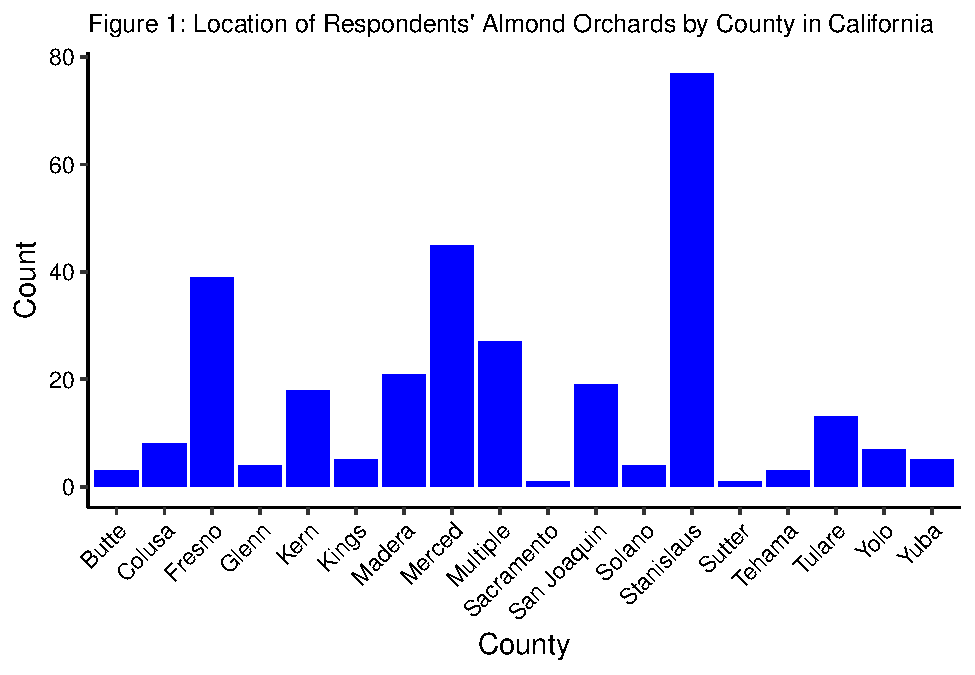
\includegraphics{Project_Template_files/figure-latex/location plots-1.pdf}
\caption{Location of Respondents' Almond Orchards by County in
California}
\end{figure}

\newpage

\textbf{Figure 2} plots the location of the respondents' almond orchards
by region. We can see from this plot that a majority of the respondents
farm almonds in the San Joaquin and Tulare Basins. It is important to
note that the northern section of the Central Valley consists of the
Sacramento Valley and Delta regions, while the southern section includes
the San Joaquin and Tulare Basins. Therefore, a majority of the
respondents farm almonds in the southern section of the Central Valley.

\begin{figure}
\centering
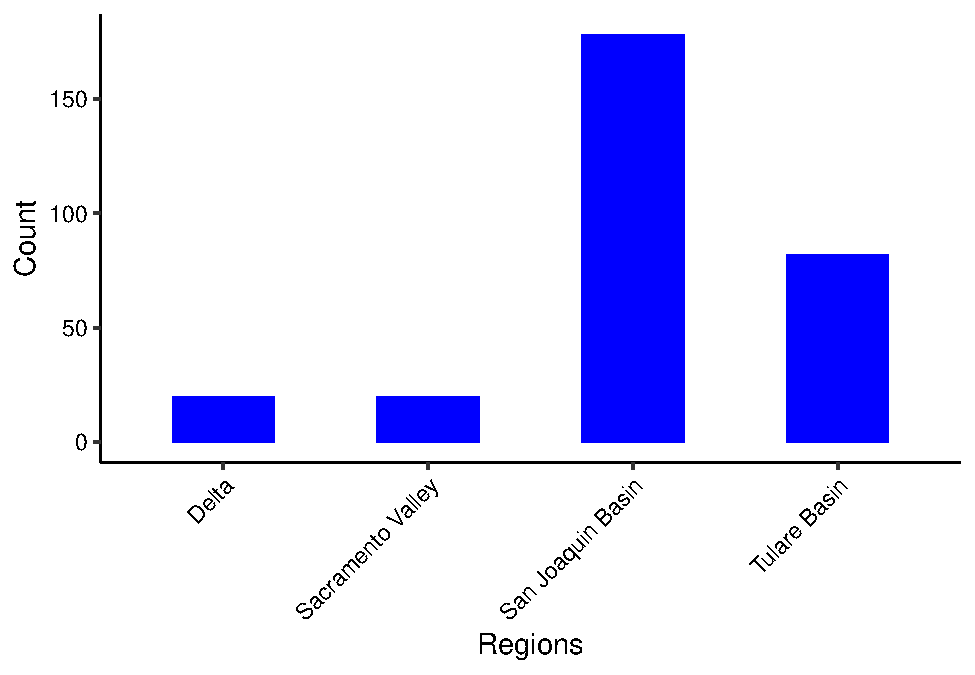
\includegraphics{Project_Template_files/figure-latex/unnamed-chunk-3-1.pdf}
\caption{Location of Respondents' Almond Orchards by Region}
\end{figure}

\newpage

\textbf{Figure 3} shows the age ranges of the respondents who completed
the survey. We can see from this plot that a majority of the respondents
fell within the 25-34 and 55-64-year-old age ranges. These age ranges
are interesting to note because the responses for cover crop adoption
will be come from both the newer and older farming generations.

\begin{figure}
\centering
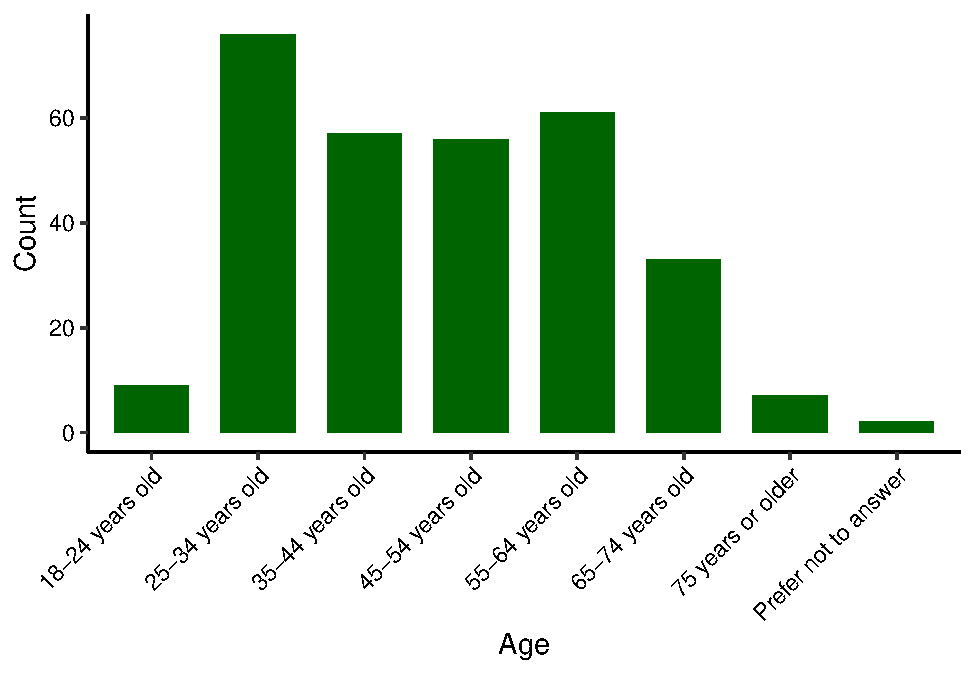
\includegraphics{Project_Template_files/figure-latex/respondent age-1.pdf}
\caption{Age Ranges of Respondents}
\end{figure}

\textbf{Figure 4} plots the respondents' roles in almond operations. The
respondents could select ``Owner, not responsible for dat-to-day
management,'' ``Owner/Operator,'' or ``Farm Manager (not owner).'' This
figure shows that a majority of the respondents selected
``Owner/Operator,'' meaning they own and operate their almond
orchard(s). This outcome was the opposite of my hypothesis regarding the
roles the survey takers play in day-to-day operations because I assumed
that a majority of the farms would consist of several parcels that were
operated by farm managers and that farm managers would constitute the
majority of survey respondents.

\begin{figure}
\centering
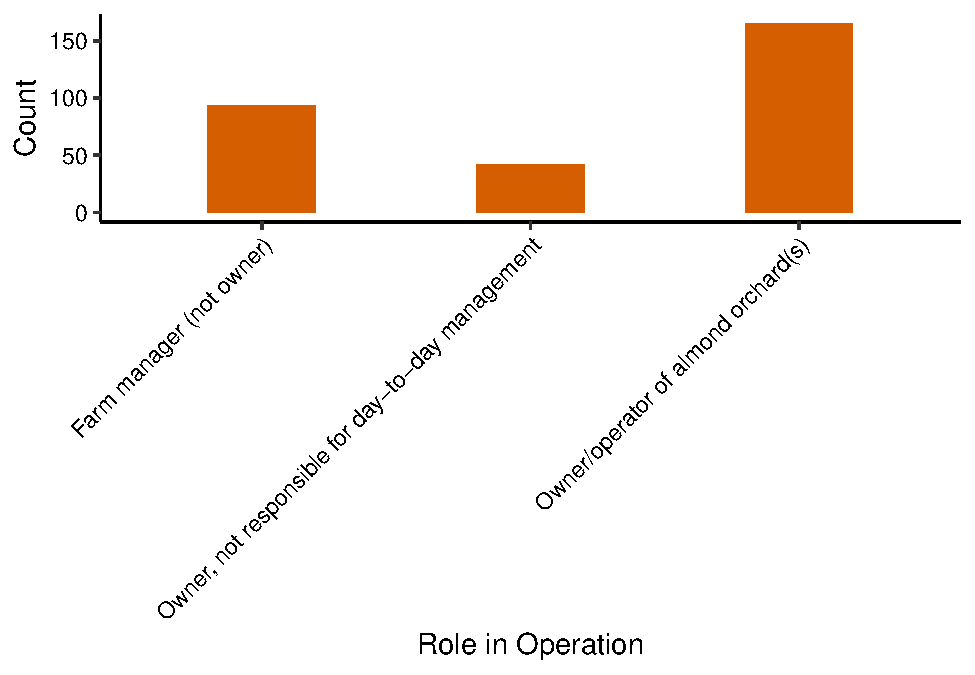
\includegraphics{Project_Template_files/figure-latex/Role in Operation-1.pdf}
\caption{Respondents' Roles in Almond Operations}
\end{figure}

\newpage

\section{Analysis}\label{analysis}

Analyzing possible factors affecting cover crop adoption among almond
producers in California will allow me to obtain a greater insight into
barriers that may be preventing producers from adopting cover crop and
thus, bee-friendly practices. To assess cover crop adoption, I analyzed
whether or not the respondents had grown a cover crop in the last five
years. Out of 301 responses, 33.6\% (101 respondents) answered ``Yes''
to having grown a cover crop, while 66.5\% (200) selected ``No.'' To
understand why respondents may have selected ``No'' or ``Not Sure'' when
asked whether they had grown a cover crop, I analyzed how responses
differed by demographics using logistic regressions and chi-square tests
of independence.

When controlling for all factors, we see that respondents who farm
almonds in the San Joaquin and Tulare Basins are significantly less
likely to grow a cover crop than respondents from the Delta (glm; z =
-3.32, p-value \textless{} 0.05; glm; z = -3.66, p-value \textless{}
0.05). We also see that that total yield-bearing acreage has a
signficant affect on whether or not respondents grow cover crop (glm; z
= -1.97, p-value \textless{} 0.05). Lastly, results indicate that there
is a marginally significant liklihood of Owner/Operators selecting
``Yes'' to having grown cover crop over Farm Managers (glm; z = -1.94,
p-value = 0.053).

\subsection{Question 1: Which demographic factors affect whether or not
respondents have planted cover crop in the last 5
years?}\label{question-1-which-demographic-factors-affect-whether-or-not-respondents-have-planted-cover-crop-in-the-last-5-years}

\begin{Shaded}
\begin{Highlighting}[]
\CommentTok{# Number of respondents who have grown and not grown a cover crop grown }

\NormalTok{CCtbl <-}\StringTok{ }\KeywordTok{table}\NormalTok{(almonds.CC}\OperatorTok{$}\NormalTok{Cover.Crop.Grown)}

\NormalTok{CCtbl}
\end{Highlighting}
\end{Shaded}

\begin{verbatim}
## 
##  No Yes 
## 200 101
\end{verbatim}

\begin{Shaded}
\begin{Highlighting}[]
\CommentTok{# Statistical Test 1: GLM}

\NormalTok{almonds.CC}\OperatorTok{$}\NormalTok{Total.Yield.Bearing.Acreage <-}\StringTok{ }
\StringTok{  }\KeywordTok{as.numeric}\NormalTok{(almonds.CC}\OperatorTok{$}\NormalTok{Total.Yield.Bearing.Acreage)}

\NormalTok{Grown.CC <-}\StringTok{ }\KeywordTok{glm}\NormalTok{(Cover.Crop.Grown }\OperatorTok{~}\StringTok{ }\KeywordTok{as.factor}\NormalTok{(Regions) }\OperatorTok{+}\StringTok{ }
\StringTok{                  }\KeywordTok{as.factor}\NormalTok{(Role.in.Operation) }\OperatorTok{+}\StringTok{ }\KeywordTok{as.factor}\NormalTok{(Age)}
               \OperatorTok{+}\StringTok{ }\NormalTok{Total.Yield.Bearing.Acreage, almonds.CC, }\DataTypeTok{family =}\NormalTok{ binomial)}

\KeywordTok{summ}\NormalTok{(Grown.CC, }\DataTypeTok{model.fit =} \KeywordTok{getOption}\NormalTok{(}\StringTok{"Grown.CC"}\NormalTok{, }\OtherTok{TRUE}\NormalTok{))}
\end{Highlighting}
\end{Shaded}

\begin{table}[!h]
\centering
\begin{tabular}{lr}
\toprule
\rowcolor{gray!6}  Observations & 300 (1 missing obs. deleted)\\
Dependent variable & Cover.Crop.Grown\\
\rowcolor{gray!6}  Type & Generalized linear model\\
Family & binomial\\
\rowcolor{gray!6}  Link & logit\\
\bottomrule
\end{tabular}
\end{table}

\begin{table}[!h]
\centering
\begin{tabular}{lr}
\toprule
\rowcolor{gray!6}  $\chi^2$(13) & 38.10\\
Pseudo-R² (Cragg-Uhler) & 0.17\\
\rowcolor{gray!6}  Pseudo-R² (McFadden) & 0.10\\
AIC & 373.18\\
\rowcolor{gray!6}  BIC & 425.04\\
\bottomrule
\end{tabular}
\end{table}

\begin{table}[!h]
\centering
\begin{threeparttable}
\begin{tabular}{lrrrr}
\toprule
  & Est. & S.E. & z val. & p\\
\midrule
\rowcolor{gray!6}  (Intercept) & 0.67 & 1.00 & 0.67 & 0.50\\
as.factor(Regions)Sacramento Valley & -0.43 & 0.71 & -0.61 & 0.54\\
\rowcolor{gray!6}  as.factor(Regions)San Joaquin Basin & -1.83 & 0.55 & -3.32 & 0.00\\
as.factor(Regions)Tulare Basin & -2.15 & 0.59 & -3.66 & 0.00\\
\rowcolor{gray!6}  as.factor(Role.in.Operation)Owner, not responsible for day-to-day management & -0.50 & 0.43 & -1.16 & 0.25\\
\addlinespace
as.factor(Role.in.Operation)Owner/operator of almond orchard(s) & -0.61 & 0.32 & -1.94 & 0.05\\
\rowcolor{gray!6}  as.factor(Age)25-34 years old & 0.70 & 0.97 & 0.72 & 0.47\\
as.factor(Age)35-44 years old & 1.54 & 0.98 & 1.57 & 0.12\\
\rowcolor{gray!6}  as.factor(Age)45-54 years old & 1.38 & 0.98 & 1.41 & 0.16\\
as.factor(Age)55-64 years old & 1.46 & 0.99 & 1.48 & 0.14\\
\addlinespace
\rowcolor{gray!6}  as.factor(Age)65-74 years old & 0.88 & 1.02 & 0.86 & 0.39\\
as.factor(Age)75 years or older & 0.43 & 1.44 & 0.30 & 0.77\\
\rowcolor{gray!6}  as.factor(Age)Prefer not to answer & -12.24 & 618.25 & -0.02 & 0.98\\
Total.Yield.Bearing.Acreage & -0.01 & 0.00 & -1.97 & 0.05\\
\bottomrule
\end{tabular}
\begin{tablenotes}
\item Standard errors: MLE
\end{tablenotes}
\end{threeparttable}
\end{table}

\begin{Shaded}
\begin{Highlighting}[]
\CommentTok{# Table 1}

\NormalTok{pretty_GrownCC.glm <-}\StringTok{ }\KeywordTok{prettify}\NormalTok{(}\KeywordTok{summary}\NormalTok{(Grown.CC))}
\end{Highlighting}
\end{Shaded}

\begin{verbatim}
## Waiting for profiling to be done...
\end{verbatim}

\begin{Shaded}
\begin{Highlighting}[]
\KeywordTok{kable}\NormalTok{(pretty_GrownCC.glm,}\DataTypeTok{caption =} \StringTok{"Cover Crop Adoption by Respondent Demographics"}\NormalTok{, }
      \DataTypeTok{align =} \KeywordTok{c}\NormalTok{(}\StringTok{"l"}\NormalTok{, }\KeywordTok{rep}\NormalTok{(}\StringTok{"r"}\NormalTok{, }\DecValTok{3}\NormalTok{)),}\DataTypeTok{format =} \StringTok{"latex"}\NormalTok{, }\DataTypeTok{booktabs =} \OtherTok{TRUE}\NormalTok{)  }\OperatorTok
\StringTok{  }\KeywordTok{kable_styling}\NormalTok{(}\DataTypeTok{latex_options =} \StringTok{"scale_down"}\NormalTok{)}
\end{Highlighting}
\end{Shaded}

\begin{table}

\caption{\label{tab:unnamed-chunk-4}Cover Crop Adoption by Respondent Demographics}
\centering
\resizebox{\linewidth}{!}{
\begin{tabular}[t]{lrrrlrrrl}
\toprule
  & Estimate & Odds Ratio & CI (lower) & CI (upper) & Std. Error & z value & Pr(>|z|) &    \\
\midrule
(Intercept) & 0.6735526 & 1.9611924 & 0.2276019 & 1.343706e+01 & 0.9992537 & 0.6740557 & 0.5 & \\
as.factor(Regions)Sacramento Valley & -0.4331810 & 0.6484431 & 0.1562540 & 2.601697e+00 & 0.7089666 & -0.6110034 & 0.541 & \\
as.factor(Regions)San Joaquin Basin & -1.8264889 & 0.1609778 & 0.0506884 & 4.538400e-01 & 0.5509155 & -3.3153706 & 0.001 & ***\\
as.factor(Regions)Tulare Basin & -2.1465417 & 0.1168877 & 0.0344185 & 3.522543e-01 & 0.5862495 & -3.6614816 & <0.001 & ***\\
as.factor(Role.in.Operation)Owner, not responsible for day-to-day management & -0.5014137 & 0.6056738 & 0.2535697 & 1.396341e+00 & 0.4330734 & -1.1578030 & 0.247 & \\
\addlinespace
as.factor(Role.in.Operation)Owner/operator of almond orchard(s) & -0.6106427 & 0.5430018 & 0.2912510 & 1.005196e+00 & 0.3150897 & -1.9379961 & 0.053 & .\\
as.factor(Age)25-34 years old & 0.6963671 & 2.0064502 & 0.3562549 & 1.770932e+01 & 0.9658172 & 0.7210133 & 0.471 & \\
as.factor(Age)35-44 years old & 1.5372192 & 4.6516371 & 0.8120775 & 4.217531e+01 & 0.9784133 & 1.5711349 & 0.116 & \\
as.factor(Age)45-54 years old & 1.3796698 & 3.9735894 & 0.6894595 & 3.589636e+01 & 0.9786013 & 1.4098385 & 0.159 & \\
as.factor(Age)55-64 years old & 1.4569459 & 4.2928287 & 0.7402873 & 3.940042e+01 & 0.9851822 & 1.4788594 & 0.139 & \\
\addlinespace
as.factor(Age)65-74 years old & 0.8814707 & 2.4144480 & 0.3747732 & 2.331597e+01 & 1.0243793 & 0.8604925 & 0.39 & \\
as.factor(Age)75 years or older & 0.4265512 & 1.5319649 & 0.0553530 & 2.532588e+01 & 1.4411770 & 0.2959742 & 0.767 & \\
as.factor(Age)Prefer not to answer & -12.2354867 & 0.0000049 & NA & 1.324559e+28 & 618.2538111 & -0.0197904 & 0.984 & \\
Total.Yield.Bearing.Acreage & -0.0072510 & 0.9927752 & 0.9854897 & 9.998687e-01 & 0.0036844 & -1.9680474 & 0.049 & *\\
\bottomrule
\end{tabular}}
\end{table}

\subsection{Question 2: How does the respondent's role in the operation
affect whether or not they have grown cover crop in the last 5
years?}\label{question-2-how-does-the-respondents-role-in-the-operation-affect-whether-or-not-they-have-grown-cover-crop-in-the-last-5-years}

To analyze how the respondent's ``role in operation'' affects whether or
not they have grown a cover crop, I first made a plot to visualize the
number of farm managers, owners, and owner/operators who have and have
not grown cover crop in the last five years. \textbf{Figure 5}
illustrates that the majority of respondents owned and operated their
almond operation, and a majority of them have not grown cover crop.

\begin{Shaded}
\begin{Highlighting}[]
\NormalTok{alm.Role=}\StringTok{ }\NormalTok{almonds.CC[almonds.CC}\OperatorTok{$}\NormalTok{Role.in.Operation }\OperatorTok{!=}\StringTok{ " "}\NormalTok{ ,]}
\end{Highlighting}
\end{Shaded}

\FloatBarrier

  \providecommand{\huxb}[2]{\arrayrulecolor[RGB]{#1}\global\arrayrulewidth=#2pt}
  \providecommand{\huxvb}[2]{\color[RGB]{#1}\vrule width #2pt}
  \providecommand{\huxtpad}[1]{\rule{0pt}{\baselineskip+#1}}
  \providecommand{\huxbpad}[1]{\rule[-#1]{0pt}{#1}}

\begin{table}[h]
\begin{raggedright}
\begin{threeparttable}
\begin{tabularx}{0.6\textwidth}{p{0.2\textwidth} p{0.2\textwidth} p{0.2\textwidth}}


\hhline{>{\huxb{0, 0, 0}{0.4}}->{\huxb{0, 0, 0}{0.4}}->{\huxb{0, 0, 0}{0.4}}-}
\arrayrulecolor{black}

\multicolumn{1}{!{\huxvb{0, 0, 0}{0.4}}l!{\huxvb{0, 0, 0}{0}}}{\huxtpad{4pt}\raggedright \textbf{alm.Role.Role.in.Operation}\huxbpad{4pt}} &
\multicolumn{1}{l!{\huxvb{0, 0, 0}{0}}}{\huxtpad{4pt}\raggedright \textbf{alm.Role.Cover.Crop.Grown}\huxbpad{4pt}} &
\multicolumn{1}{r!{\huxvb{0, 0, 0}{0.4}}}{\huxtpad{4pt}\raggedleft \textbf{Freq}\huxbpad{4pt}} \tabularnewline[-0.5pt]


\hhline{>{\huxb{0, 0, 0}{0.4}}->{\huxb{0, 0, 0}{0.4}}->{\huxb{0, 0, 0}{0.4}}-}
\arrayrulecolor{black}

\multicolumn{1}{!{\huxvb{0, 0, 0}{0.4}}p{0.2\textwidth}!{\huxvb{0, 0, 0}{0}}}{\cellcolor[RGB]{242, 242, 242}\parbox[b]{0.2\textwidth-4pt-4pt}{\huxtpad{4pt}\raggedright Farm manager (not owner)\huxbpad{4pt}}} &
\multicolumn{1}{l!{\huxvb{0, 0, 0}{0}}}{\cellcolor[RGB]{242, 242, 242}\huxtpad{4pt}\raggedright No\huxbpad{4pt}} &
\multicolumn{1}{r!{\huxvb{0, 0, 0}{0.4}}}{\cellcolor[RGB]{242, 242, 242}\huxtpad{4pt}\raggedleft 57\huxbpad{4pt}} \tabularnewline[-0.5pt]


\hhline{>{\huxb{0, 0, 0}{0.4}}|>{\huxb{0, 0, 0}{0.4}}|}
\arrayrulecolor{black}

\multicolumn{1}{!{\huxvb{0, 0, 0}{0.4}}p{0.2\textwidth}!{\huxvb{0, 0, 0}{0}}}{\parbox[b]{0.2\textwidth-4pt-4pt}{\huxtpad{4pt}\raggedright Owner, not responsible for day-to-day management\huxbpad{4pt}}} &
\multicolumn{1}{l!{\huxvb{0, 0, 0}{0}}}{\huxtpad{4pt}\raggedright No\huxbpad{4pt}} &
\multicolumn{1}{r!{\huxvb{0, 0, 0}{0.4}}}{\huxtpad{4pt}\raggedleft 28\huxbpad{4pt}} \tabularnewline[-0.5pt]


\hhline{>{\huxb{0, 0, 0}{0.4}}|>{\huxb{0, 0, 0}{0.4}}|}
\arrayrulecolor{black}

\multicolumn{1}{!{\huxvb{0, 0, 0}{0.4}}p{0.2\textwidth}!{\huxvb{0, 0, 0}{0}}}{\cellcolor[RGB]{242, 242, 242}\parbox[b]{0.2\textwidth-4pt-4pt}{\huxtpad{4pt}\raggedright Owner/operator of almond orchard(s)\huxbpad{4pt}}} &
\multicolumn{1}{l!{\huxvb{0, 0, 0}{0}}}{\cellcolor[RGB]{242, 242, 242}\huxtpad{4pt}\raggedright No\huxbpad{4pt}} &
\multicolumn{1}{r!{\huxvb{0, 0, 0}{0.4}}}{\cellcolor[RGB]{242, 242, 242}\huxtpad{4pt}\raggedleft 115\huxbpad{4pt}} \tabularnewline[-0.5pt]


\hhline{>{\huxb{0, 0, 0}{0.4}}|>{\huxb{0, 0, 0}{0.4}}|}
\arrayrulecolor{black}

\multicolumn{1}{!{\huxvb{0, 0, 0}{0.4}}p{0.2\textwidth}!{\huxvb{0, 0, 0}{0}}}{\parbox[b]{0.2\textwidth-4pt-4pt}{\huxtpad{4pt}\raggedright Farm manager (not owner)\huxbpad{4pt}}} &
\multicolumn{1}{l!{\huxvb{0, 0, 0}{0}}}{\huxtpad{4pt}\raggedright Yes\huxbpad{4pt}} &
\multicolumn{1}{r!{\huxvb{0, 0, 0}{0.4}}}{\huxtpad{4pt}\raggedleft 37\huxbpad{4pt}} \tabularnewline[-0.5pt]


\hhline{>{\huxb{0, 0, 0}{0.4}}|>{\huxb{0, 0, 0}{0.4}}|}
\arrayrulecolor{black}

\multicolumn{1}{!{\huxvb{0, 0, 0}{0.4}}p{0.2\textwidth}!{\huxvb{0, 0, 0}{0}}}{\cellcolor[RGB]{242, 242, 242}\parbox[b]{0.2\textwidth-4pt-4pt}{\huxtpad{4pt}\raggedright Owner, not responsible for day-to-day management\huxbpad{4pt}}} &
\multicolumn{1}{l!{\huxvb{0, 0, 0}{0}}}{\cellcolor[RGB]{242, 242, 242}\huxtpad{4pt}\raggedright Yes\huxbpad{4pt}} &
\multicolumn{1}{r!{\huxvb{0, 0, 0}{0.4}}}{\cellcolor[RGB]{242, 242, 242}\huxtpad{4pt}\raggedleft 14\huxbpad{4pt}} \tabularnewline[-0.5pt]


\hhline{>{\huxb{0, 0, 0}{0.4}}|>{\huxb{0, 0, 0}{0.4}}|}
\arrayrulecolor{black}

\multicolumn{1}{!{\huxvb{0, 0, 0}{0.4}}p{0.2\textwidth}!{\huxvb{0, 0, 0}{0}}}{\parbox[b]{0.2\textwidth-4pt-4pt}{\huxtpad{4pt}\raggedright Owner/operator of almond orchard(s)\huxbpad{4pt}}} &
\multicolumn{1}{l!{\huxvb{0, 0, 0}{0}}}{\huxtpad{4pt}\raggedright Yes\huxbpad{4pt}} &
\multicolumn{1}{r!{\huxvb{0, 0, 0}{0.4}}}{\huxtpad{4pt}\raggedleft 50\huxbpad{4pt}} \tabularnewline[-0.5pt]


\hhline{>{\huxb{0, 0, 0}{0.4}}->{\huxb{0, 0, 0}{0.4}}->{\huxb{0, 0, 0}{0.4}}-}
\arrayrulecolor{black}
\end{tabularx}\end{threeparttable}
\par\end{raggedright}

\end{table}

\begin{figure}
\centering
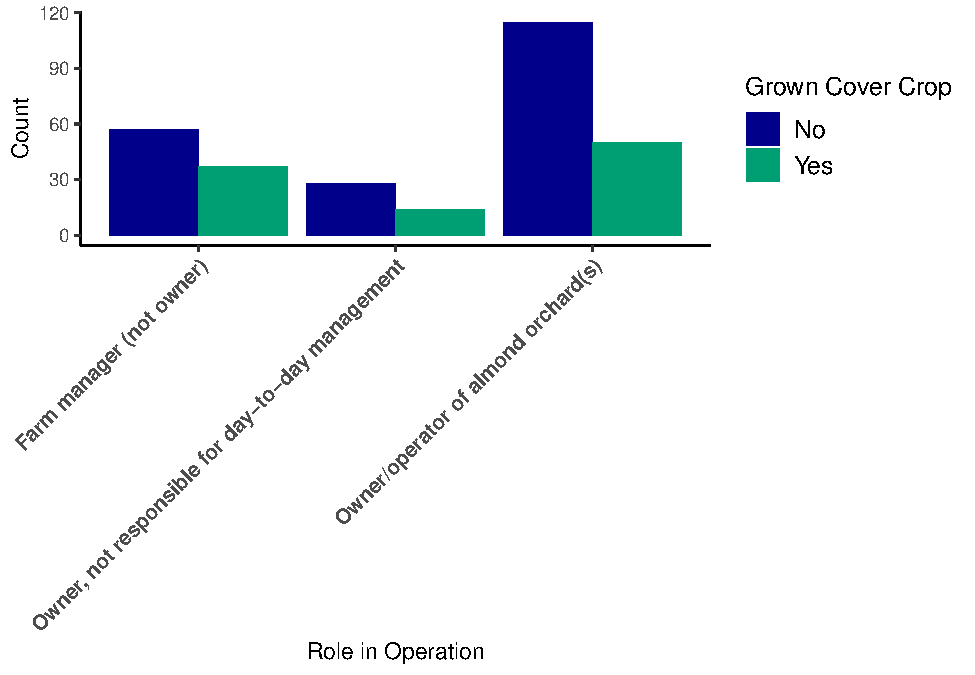
\includegraphics{Project_Template_files/figure-latex/Question 2 Plot-1.pdf}
\caption{Respondents' Roles in Almond Operations by Cover Crop Grown}
\end{figure}

\FloatBarrier

I then performed a chi-square test of independence to examine the
relationship between ``role in operation'' and whether or not a
respondent grew a cover crop. I found that the two variables are
independent - a respondent's ``role in operation'' does not
significantly affect whether or not they had grown cover crop in the
last five years (X\^{}2(2, N = 301) = 2.21, p \textgreater{} 0.05).

\begin{Shaded}
\begin{Highlighting}[]
\CommentTok{# Statistical Test 1: Chi-square}

\NormalTok{almonds.numeric}\OperatorTok{$}\NormalTok{Role.in.Operation <-}\StringTok{ }\KeywordTok{as.factor}\NormalTok{(almonds.numeric}\OperatorTok{$}\NormalTok{Role.in.Operation)}
\NormalTok{almonds.numeric}\OperatorTok{$}\NormalTok{Cover.Crop.Grown <-}\StringTok{ }\KeywordTok{as.factor}\NormalTok{(almonds.numeric}\OperatorTok{$}\NormalTok{Cover.Crop.Grown)}



\NormalTok{Role.Grown.CC.tbl =}\StringTok{ }\KeywordTok{table}\NormalTok{(almonds.numeric}\OperatorTok{$}\NormalTok{Role.in.Operatio, }
\NormalTok{                          almonds.numeric}\OperatorTok{$}\NormalTok{Cover.Crop.Grown) }
\NormalTok{Role.Grown.CC.tbl}
\end{Highlighting}
\end{Shaded}

\begin{verbatim}
##    
##       1   2
##   1  14  28
##   2  50 115
##   3  37  57
\end{verbatim}

\begin{Shaded}
\begin{Highlighting}[]
\KeywordTok{chisq.test}\NormalTok{(Role.Grown.CC.tbl)}
\end{Highlighting}
\end{Shaded}

\begin{verbatim}
## 
##  Pearson's Chi-squared test
## 
## data:  Role.Grown.CC.tbl
## X-squared = 2.2051, df = 2, p-value = 0.332
\end{verbatim}

\subsection{Question 3: How does the respondent's age affect whether or
not they have grown cover crop in the last 5
years?}\label{question-3-how-does-the-respondents-age-affect-whether-or-not-they-have-grown-cover-crop-in-the-last-5-years}

I first plotted the age of respondents by whether or not they have grown
a cover crop to visualize the relationship between the two variables.
Graph ``a'' in \textbf{Figure 6} shows that respondents between
55-64-years-old had the highest frequency of growing cover crop in the
last five years, while respondents between 25-34-years-old had the
highest frequency of \textbf{not} growing cover crop in the last five
years. The higher rate of respondents between 25-34-years-old not having
grown cover crop may be due to the fact that they have just purchased
the almond orchards or are farm managers, whereas the older generation
has most likely been farming for a longer period of time. However, I
hypothesize that a greater number of respondents between 25-34-years-old
would be interested in growing cover crop than older respondents.

  \providecommand{\huxb}[2]{\arrayrulecolor[RGB]{#1}\global\arrayrulewidth=#2pt}
  \providecommand{\huxvb}[2]{\color[RGB]{#1}\vrule width #2pt}
  \providecommand{\huxtpad}[1]{\rule{0pt}{\baselineskip+#1}}
  \providecommand{\huxbpad}[1]{\rule[-#1]{0pt}{#1}}

\begin{table}[h]
\begin{raggedright}
\begin{threeparttable}
\begin{tabularx}{0.277777777777778\textwidth}{p{0.0925925925925926\textwidth} p{0.0925925925925926\textwidth} p{0.0925925925925926\textwidth}}


\hhline{>{\huxb{0, 0, 0}{0.4}}->{\huxb{0, 0, 0}{0.4}}->{\huxb{0, 0, 0}{0.4}}-}
\arrayrulecolor{black}

\multicolumn{1}{!{\huxvb{0, 0, 0}{0.4}}l!{\huxvb{0, 0, 0}{0}}}{\huxtpad{4pt}\raggedright \textbf{almAge.Age}\huxbpad{4pt}} &
\multicolumn{1}{l!{\huxvb{0, 0, 0}{0}}}{\huxtpad{4pt}\raggedright \textbf{almAge.Cover.Crop.Grown}\huxbpad{4pt}} &
\multicolumn{1}{r!{\huxvb{0, 0, 0}{0.4}}}{\huxtpad{4pt}\raggedleft \textbf{Freq}\huxbpad{4pt}} \tabularnewline[-0.5pt]


\hhline{>{\huxb{0, 0, 0}{0.4}}->{\huxb{0, 0, 0}{0.4}}->{\huxb{0, 0, 0}{0.4}}-}
\arrayrulecolor{black}

\multicolumn{1}{!{\huxvb{0, 0, 0}{0.4}}p{0.0925925925925926\textwidth}!{\huxvb{0, 0, 0}{0}}}{\cellcolor[RGB]{242, 242, 242}\parbox[b]{0.0925925925925926\textwidth-4pt-4pt}{\huxtpad{4pt}\raggedright 18-24 years old\huxbpad{4pt}}} &
\multicolumn{1}{l!{\huxvb{0, 0, 0}{0}}}{\cellcolor[RGB]{242, 242, 242}\huxtpad{4pt}\raggedright No\huxbpad{4pt}} &
\multicolumn{1}{r!{\huxvb{0, 0, 0}{0.4}}}{\cellcolor[RGB]{242, 242, 242}\huxtpad{4pt}\raggedleft 7\huxbpad{4pt}} \tabularnewline[-0.5pt]


\hhline{>{\huxb{0, 0, 0}{0.4}}|>{\huxb{0, 0, 0}{0.4}}|}
\arrayrulecolor{black}

\multicolumn{1}{!{\huxvb{0, 0, 0}{0.4}}p{0.0925925925925926\textwidth}!{\huxvb{0, 0, 0}{0}}}{\parbox[b]{0.0925925925925926\textwidth-4pt-4pt}{\huxtpad{4pt}\raggedright 25-34 years old\huxbpad{4pt}}} &
\multicolumn{1}{l!{\huxvb{0, 0, 0}{0}}}{\huxtpad{4pt}\raggedright No\huxbpad{4pt}} &
\multicolumn{1}{r!{\huxvb{0, 0, 0}{0.4}}}{\huxtpad{4pt}\raggedleft 56\huxbpad{4pt}} \tabularnewline[-0.5pt]


\hhline{>{\huxb{0, 0, 0}{0.4}}|>{\huxb{0, 0, 0}{0.4}}|}
\arrayrulecolor{black}

\multicolumn{1}{!{\huxvb{0, 0, 0}{0.4}}p{0.0925925925925926\textwidth}!{\huxvb{0, 0, 0}{0}}}{\cellcolor[RGB]{242, 242, 242}\parbox[b]{0.0925925925925926\textwidth-4pt-4pt}{\huxtpad{4pt}\raggedright 35-44 years old\huxbpad{4pt}}} &
\multicolumn{1}{l!{\huxvb{0, 0, 0}{0}}}{\cellcolor[RGB]{242, 242, 242}\huxtpad{4pt}\raggedright No\huxbpad{4pt}} &
\multicolumn{1}{r!{\huxvb{0, 0, 0}{0.4}}}{\cellcolor[RGB]{242, 242, 242}\huxtpad{4pt}\raggedleft 34\huxbpad{4pt}} \tabularnewline[-0.5pt]


\hhline{>{\huxb{0, 0, 0}{0.4}}|>{\huxb{0, 0, 0}{0.4}}|}
\arrayrulecolor{black}

\multicolumn{1}{!{\huxvb{0, 0, 0}{0.4}}p{0.0925925925925926\textwidth}!{\huxvb{0, 0, 0}{0}}}{\parbox[b]{0.0925925925925926\textwidth-4pt-4pt}{\huxtpad{4pt}\raggedright 45-54 years old\huxbpad{4pt}}} &
\multicolumn{1}{l!{\huxvb{0, 0, 0}{0}}}{\huxtpad{4pt}\raggedright No\huxbpad{4pt}} &
\multicolumn{1}{r!{\huxvb{0, 0, 0}{0.4}}}{\huxtpad{4pt}\raggedleft 33\huxbpad{4pt}} \tabularnewline[-0.5pt]


\hhline{>{\huxb{0, 0, 0}{0.4}}|>{\huxb{0, 0, 0}{0.4}}|}
\arrayrulecolor{black}

\multicolumn{1}{!{\huxvb{0, 0, 0}{0.4}}p{0.0925925925925926\textwidth}!{\huxvb{0, 0, 0}{0}}}{\cellcolor[RGB]{242, 242, 242}\parbox[b]{0.0925925925925926\textwidth-4pt-4pt}{\huxtpad{4pt}\raggedright 55-64 years old\huxbpad{4pt}}} &
\multicolumn{1}{l!{\huxvb{0, 0, 0}{0}}}{\cellcolor[RGB]{242, 242, 242}\huxtpad{4pt}\raggedright No\huxbpad{4pt}} &
\multicolumn{1}{r!{\huxvb{0, 0, 0}{0.4}}}{\cellcolor[RGB]{242, 242, 242}\huxtpad{4pt}\raggedleft 38\huxbpad{4pt}} \tabularnewline[-0.5pt]


\hhline{>{\huxb{0, 0, 0}{0.4}}|>{\huxb{0, 0, 0}{0.4}}|}
\arrayrulecolor{black}

\multicolumn{1}{!{\huxvb{0, 0, 0}{0.4}}p{0.0925925925925926\textwidth}!{\huxvb{0, 0, 0}{0}}}{\parbox[b]{0.0925925925925926\textwidth-4pt-4pt}{\huxtpad{4pt}\raggedright 65-74 years old\huxbpad{4pt}}} &
\multicolumn{1}{l!{\huxvb{0, 0, 0}{0}}}{\huxtpad{4pt}\raggedright No\huxbpad{4pt}} &
\multicolumn{1}{r!{\huxvb{0, 0, 0}{0.4}}}{\huxtpad{4pt}\raggedleft 24\huxbpad{4pt}} \tabularnewline[-0.5pt]


\hhline{>{\huxb{0, 0, 0}{0.4}}|>{\huxb{0, 0, 0}{0.4}}|}
\arrayrulecolor{black}

\multicolumn{1}{!{\huxvb{0, 0, 0}{0.4}}p{0.0925925925925926\textwidth}!{\huxvb{0, 0, 0}{0}}}{\cellcolor[RGB]{242, 242, 242}\parbox[b]{0.0925925925925926\textwidth-4pt-4pt}{\huxtpad{4pt}\raggedright 75 years or older\huxbpad{4pt}}} &
\multicolumn{1}{l!{\huxvb{0, 0, 0}{0}}}{\cellcolor[RGB]{242, 242, 242}\huxtpad{4pt}\raggedright No\huxbpad{4pt}} &
\multicolumn{1}{r!{\huxvb{0, 0, 0}{0.4}}}{\cellcolor[RGB]{242, 242, 242}\huxtpad{4pt}\raggedleft 6\huxbpad{4pt}} \tabularnewline[-0.5pt]


\hhline{>{\huxb{0, 0, 0}{0.4}}|>{\huxb{0, 0, 0}{0.4}}|}
\arrayrulecolor{black}

\multicolumn{1}{!{\huxvb{0, 0, 0}{0.4}}p{0.0925925925925926\textwidth}!{\huxvb{0, 0, 0}{0}}}{\parbox[b]{0.0925925925925926\textwidth-4pt-4pt}{\huxtpad{4pt}\raggedright Prefer not to answer\huxbpad{4pt}}} &
\multicolumn{1}{l!{\huxvb{0, 0, 0}{0}}}{\huxtpad{4pt}\raggedright No\huxbpad{4pt}} &
\multicolumn{1}{r!{\huxvb{0, 0, 0}{0.4}}}{\huxtpad{4pt}\raggedleft 2\huxbpad{4pt}} \tabularnewline[-0.5pt]


\hhline{>{\huxb{0, 0, 0}{0.4}}|>{\huxb{0, 0, 0}{0.4}}|}
\arrayrulecolor{black}

\multicolumn{1}{!{\huxvb{0, 0, 0}{0.4}}p{0.0925925925925926\textwidth}!{\huxvb{0, 0, 0}{0}}}{\cellcolor[RGB]{242, 242, 242}\parbox[b]{0.0925925925925926\textwidth-4pt-4pt}{\huxtpad{4pt}\raggedright 18-24 years old\huxbpad{4pt}}} &
\multicolumn{1}{l!{\huxvb{0, 0, 0}{0}}}{\cellcolor[RGB]{242, 242, 242}\huxtpad{4pt}\raggedright Yes\huxbpad{4pt}} &
\multicolumn{1}{r!{\huxvb{0, 0, 0}{0.4}}}{\cellcolor[RGB]{242, 242, 242}\huxtpad{4pt}\raggedleft 2\huxbpad{4pt}} \tabularnewline[-0.5pt]


\hhline{>{\huxb{0, 0, 0}{0.4}}|>{\huxb{0, 0, 0}{0.4}}|}
\arrayrulecolor{black}

\multicolumn{1}{!{\huxvb{0, 0, 0}{0.4}}p{0.0925925925925926\textwidth}!{\huxvb{0, 0, 0}{0}}}{\parbox[b]{0.0925925925925926\textwidth-4pt-4pt}{\huxtpad{4pt}\raggedright 25-34 years old\huxbpad{4pt}}} &
\multicolumn{1}{l!{\huxvb{0, 0, 0}{0}}}{\huxtpad{4pt}\raggedright Yes\huxbpad{4pt}} &
\multicolumn{1}{r!{\huxvb{0, 0, 0}{0.4}}}{\huxtpad{4pt}\raggedleft 20\huxbpad{4pt}} \tabularnewline[-0.5pt]


\hhline{>{\huxb{0, 0, 0}{0.4}}|>{\huxb{0, 0, 0}{0.4}}|}
\arrayrulecolor{black}

\multicolumn{1}{!{\huxvb{0, 0, 0}{0.4}}p{0.0925925925925926\textwidth}!{\huxvb{0, 0, 0}{0}}}{\cellcolor[RGB]{242, 242, 242}\parbox[b]{0.0925925925925926\textwidth-4pt-4pt}{\huxtpad{4pt}\raggedright 35-44 years old\huxbpad{4pt}}} &
\multicolumn{1}{l!{\huxvb{0, 0, 0}{0}}}{\cellcolor[RGB]{242, 242, 242}\huxtpad{4pt}\raggedright Yes\huxbpad{4pt}} &
\multicolumn{1}{r!{\huxvb{0, 0, 0}{0.4}}}{\cellcolor[RGB]{242, 242, 242}\huxtpad{4pt}\raggedleft 23\huxbpad{4pt}} \tabularnewline[-0.5pt]


\hhline{>{\huxb{0, 0, 0}{0.4}}|>{\huxb{0, 0, 0}{0.4}}|}
\arrayrulecolor{black}

\multicolumn{1}{!{\huxvb{0, 0, 0}{0.4}}p{0.0925925925925926\textwidth}!{\huxvb{0, 0, 0}{0}}}{\parbox[b]{0.0925925925925926\textwidth-4pt-4pt}{\huxtpad{4pt}\raggedright 45-54 years old\huxbpad{4pt}}} &
\multicolumn{1}{l!{\huxvb{0, 0, 0}{0}}}{\huxtpad{4pt}\raggedright Yes\huxbpad{4pt}} &
\multicolumn{1}{r!{\huxvb{0, 0, 0}{0.4}}}{\huxtpad{4pt}\raggedleft 23\huxbpad{4pt}} \tabularnewline[-0.5pt]


\hhline{>{\huxb{0, 0, 0}{0.4}}|>{\huxb{0, 0, 0}{0.4}}|}
\arrayrulecolor{black}

\multicolumn{1}{!{\huxvb{0, 0, 0}{0.4}}p{0.0925925925925926\textwidth}!{\huxvb{0, 0, 0}{0}}}{\cellcolor[RGB]{242, 242, 242}\parbox[b]{0.0925925925925926\textwidth-4pt-4pt}{\huxtpad{4pt}\raggedright 55-64 years old\huxbpad{4pt}}} &
\multicolumn{1}{l!{\huxvb{0, 0, 0}{0}}}{\cellcolor[RGB]{242, 242, 242}\huxtpad{4pt}\raggedright Yes\huxbpad{4pt}} &
\multicolumn{1}{r!{\huxvb{0, 0, 0}{0.4}}}{\cellcolor[RGB]{242, 242, 242}\huxtpad{4pt}\raggedleft 23\huxbpad{4pt}} \tabularnewline[-0.5pt]


\hhline{>{\huxb{0, 0, 0}{0.4}}|>{\huxb{0, 0, 0}{0.4}}|}
\arrayrulecolor{black}

\multicolumn{1}{!{\huxvb{0, 0, 0}{0.4}}p{0.0925925925925926\textwidth}!{\huxvb{0, 0, 0}{0}}}{\parbox[b]{0.0925925925925926\textwidth-4pt-4pt}{\huxtpad{4pt}\raggedright 65-74 years old\huxbpad{4pt}}} &
\multicolumn{1}{l!{\huxvb{0, 0, 0}{0}}}{\huxtpad{4pt}\raggedright Yes\huxbpad{4pt}} &
\multicolumn{1}{r!{\huxvb{0, 0, 0}{0.4}}}{\huxtpad{4pt}\raggedleft 9\huxbpad{4pt}} \tabularnewline[-0.5pt]


\hhline{>{\huxb{0, 0, 0}{0.4}}|>{\huxb{0, 0, 0}{0.4}}|}
\arrayrulecolor{black}

\multicolumn{1}{!{\huxvb{0, 0, 0}{0.4}}p{0.0925925925925926\textwidth}!{\huxvb{0, 0, 0}{0}}}{\cellcolor[RGB]{242, 242, 242}\parbox[b]{0.0925925925925926\textwidth-4pt-4pt}{\huxtpad{4pt}\raggedright 75 years or older\huxbpad{4pt}}} &
\multicolumn{1}{l!{\huxvb{0, 0, 0}{0}}}{\cellcolor[RGB]{242, 242, 242}\huxtpad{4pt}\raggedright Yes\huxbpad{4pt}} &
\multicolumn{1}{r!{\huxvb{0, 0, 0}{0.4}}}{\cellcolor[RGB]{242, 242, 242}\huxtpad{4pt}\raggedleft 1\huxbpad{4pt}} \tabularnewline[-0.5pt]


\hhline{>{\huxb{0, 0, 0}{0.4}}|>{\huxb{0, 0, 0}{0.4}}|}
\arrayrulecolor{black}

\multicolumn{1}{!{\huxvb{0, 0, 0}{0.4}}p{0.0925925925925926\textwidth}!{\huxvb{0, 0, 0}{0}}}{\parbox[b]{0.0925925925925926\textwidth-4pt-4pt}{\huxtpad{4pt}\raggedright Prefer not to answer\huxbpad{4pt}}} &
\multicolumn{1}{l!{\huxvb{0, 0, 0}{0}}}{\huxtpad{4pt}\raggedright Yes\huxbpad{4pt}} &
\multicolumn{1}{r!{\huxvb{0, 0, 0}{0.4}}}{\huxtpad{4pt}\raggedleft 0\huxbpad{4pt}} \tabularnewline[-0.5pt]


\hhline{>{\huxb{0, 0, 0}{0.4}}->{\huxb{0, 0, 0}{0.4}}->{\huxb{0, 0, 0}{0.4}}-}
\arrayrulecolor{black}
\end{tabularx}\end{threeparttable}
\par\end{raggedright}

\end{table}

To test my hypothesis that respondents between 24-35-years-old are more
interested in planting cover crop than the older respondents, I plotted
the age of the respondents by their \emph{interest} in growing cover
crop. It is important to note that the question regarding
\emph{interest} in growing cover crop only appeared for those who
selected \emph{no} to having grown cover crop in the last 5 years. Thus,
the total count in this analysis is lower than that of the cover crop
\emph{grown} analysis. Out of the respondents who have not grown cover
crop, graph ``b'' in \textbf{Figure 6} shows that my hypothesis was
correct and that more respondents from the 25-34 age bracket are
interested in planting cover crop than the older respondents.

  \providecommand{\huxb}[2]{\arrayrulecolor[RGB]{#1}\global\arrayrulewidth=#2pt}
  \providecommand{\huxvb}[2]{\color[RGB]{#1}\vrule width #2pt}
  \providecommand{\huxtpad}[1]{\rule{0pt}{\baselineskip+#1}}
  \providecommand{\huxbpad}[1]{\rule[-#1]{0pt}{#1}}

\begin{table}[h]
\begin{raggedright}
\begin{threeparttable}
\begin{tabularx}{0.333333333333333\textwidth}{p{0.111111111111111\textwidth} p{0.111111111111111\textwidth} p{0.111111111111111\textwidth}}


\hhline{>{\huxb{0, 0, 0}{0.4}}->{\huxb{0, 0, 0}{0.4}}->{\huxb{0, 0, 0}{0.4}}-}
\arrayrulecolor{black}

\multicolumn{1}{!{\huxvb{0, 0, 0}{0.4}}l!{\huxvb{0, 0, 0}{0}}}{\huxtpad{4pt}\raggedright \textbf{alm.Age}\huxbpad{4pt}} &
\multicolumn{1}{l!{\huxvb{0, 0, 0}{0}}}{\huxtpad{4pt}\raggedright \textbf{alm.Cover.Crop.Interest}\huxbpad{4pt}} &
\multicolumn{1}{r!{\huxvb{0, 0, 0}{0.4}}}{\huxtpad{4pt}\raggedleft \textbf{Freq}\huxbpad{4pt}} \tabularnewline[-0.5pt]


\hhline{>{\huxb{0, 0, 0}{0.4}}->{\huxb{0, 0, 0}{0.4}}->{\huxb{0, 0, 0}{0.4}}-}
\arrayrulecolor{black}

\multicolumn{1}{!{\huxvb{0, 0, 0}{0.4}}p{0.111111111111111\textwidth}!{\huxvb{0, 0, 0}{0}}}{\cellcolor[RGB]{242, 242, 242}\parbox[b]{0.111111111111111\textwidth-4pt-4pt}{\huxtpad{4pt}\raggedright 18-24 years old\huxbpad{4pt}}} &
\multicolumn{1}{l!{\huxvb{0, 0, 0}{0}}}{\cellcolor[RGB]{242, 242, 242}\huxtpad{4pt}\raggedright No\huxbpad{4pt}} &
\multicolumn{1}{r!{\huxvb{0, 0, 0}{0.4}}}{\cellcolor[RGB]{242, 242, 242}\huxtpad{4pt}\raggedleft 0\huxbpad{4pt}} \tabularnewline[-0.5pt]


\hhline{>{\huxb{0, 0, 0}{0.4}}|>{\huxb{0, 0, 0}{0.4}}|}
\arrayrulecolor{black}

\multicolumn{1}{!{\huxvb{0, 0, 0}{0.4}}p{0.111111111111111\textwidth}!{\huxvb{0, 0, 0}{0}}}{\parbox[b]{0.111111111111111\textwidth-4pt-4pt}{\huxtpad{4pt}\raggedright 25-34 years old\huxbpad{4pt}}} &
\multicolumn{1}{l!{\huxvb{0, 0, 0}{0}}}{\huxtpad{4pt}\raggedright No\huxbpad{4pt}} &
\multicolumn{1}{r!{\huxvb{0, 0, 0}{0.4}}}{\huxtpad{4pt}\raggedleft 17\huxbpad{4pt}} \tabularnewline[-0.5pt]


\hhline{>{\huxb{0, 0, 0}{0.4}}|>{\huxb{0, 0, 0}{0.4}}|}
\arrayrulecolor{black}

\multicolumn{1}{!{\huxvb{0, 0, 0}{0.4}}p{0.111111111111111\textwidth}!{\huxvb{0, 0, 0}{0}}}{\cellcolor[RGB]{242, 242, 242}\parbox[b]{0.111111111111111\textwidth-4pt-4pt}{\huxtpad{4pt}\raggedright 35-44 years old\huxbpad{4pt}}} &
\multicolumn{1}{l!{\huxvb{0, 0, 0}{0}}}{\cellcolor[RGB]{242, 242, 242}\huxtpad{4pt}\raggedright No\huxbpad{4pt}} &
\multicolumn{1}{r!{\huxvb{0, 0, 0}{0.4}}}{\cellcolor[RGB]{242, 242, 242}\huxtpad{4pt}\raggedleft 9\huxbpad{4pt}} \tabularnewline[-0.5pt]


\hhline{>{\huxb{0, 0, 0}{0.4}}|>{\huxb{0, 0, 0}{0.4}}|}
\arrayrulecolor{black}

\multicolumn{1}{!{\huxvb{0, 0, 0}{0.4}}p{0.111111111111111\textwidth}!{\huxvb{0, 0, 0}{0}}}{\parbox[b]{0.111111111111111\textwidth-4pt-4pt}{\huxtpad{4pt}\raggedright 45-54 years old\huxbpad{4pt}}} &
\multicolumn{1}{l!{\huxvb{0, 0, 0}{0}}}{\huxtpad{4pt}\raggedright No\huxbpad{4pt}} &
\multicolumn{1}{r!{\huxvb{0, 0, 0}{0.4}}}{\huxtpad{4pt}\raggedleft 13\huxbpad{4pt}} \tabularnewline[-0.5pt]


\hhline{>{\huxb{0, 0, 0}{0.4}}|>{\huxb{0, 0, 0}{0.4}}|}
\arrayrulecolor{black}

\multicolumn{1}{!{\huxvb{0, 0, 0}{0.4}}p{0.111111111111111\textwidth}!{\huxvb{0, 0, 0}{0}}}{\cellcolor[RGB]{242, 242, 242}\parbox[b]{0.111111111111111\textwidth-4pt-4pt}{\huxtpad{4pt}\raggedright 55-64 years old\huxbpad{4pt}}} &
\multicolumn{1}{l!{\huxvb{0, 0, 0}{0}}}{\cellcolor[RGB]{242, 242, 242}\huxtpad{4pt}\raggedright No\huxbpad{4pt}} &
\multicolumn{1}{r!{\huxvb{0, 0, 0}{0.4}}}{\cellcolor[RGB]{242, 242, 242}\huxtpad{4pt}\raggedleft 13\huxbpad{4pt}} \tabularnewline[-0.5pt]


\hhline{>{\huxb{0, 0, 0}{0.4}}|>{\huxb{0, 0, 0}{0.4}}|}
\arrayrulecolor{black}

\multicolumn{1}{!{\huxvb{0, 0, 0}{0.4}}p{0.111111111111111\textwidth}!{\huxvb{0, 0, 0}{0}}}{\parbox[b]{0.111111111111111\textwidth-4pt-4pt}{\huxtpad{4pt}\raggedright 65-74 years old\huxbpad{4pt}}} &
\multicolumn{1}{l!{\huxvb{0, 0, 0}{0}}}{\huxtpad{4pt}\raggedright No\huxbpad{4pt}} &
\multicolumn{1}{r!{\huxvb{0, 0, 0}{0.4}}}{\huxtpad{4pt}\raggedleft 8\huxbpad{4pt}} \tabularnewline[-0.5pt]


\hhline{>{\huxb{0, 0, 0}{0.4}}|>{\huxb{0, 0, 0}{0.4}}|}
\arrayrulecolor{black}

\multicolumn{1}{!{\huxvb{0, 0, 0}{0.4}}p{0.111111111111111\textwidth}!{\huxvb{0, 0, 0}{0}}}{\cellcolor[RGB]{242, 242, 242}\parbox[b]{0.111111111111111\textwidth-4pt-4pt}{\huxtpad{4pt}\raggedright 75 years or older\huxbpad{4pt}}} &
\multicolumn{1}{l!{\huxvb{0, 0, 0}{0}}}{\cellcolor[RGB]{242, 242, 242}\huxtpad{4pt}\raggedright No\huxbpad{4pt}} &
\multicolumn{1}{r!{\huxvb{0, 0, 0}{0.4}}}{\cellcolor[RGB]{242, 242, 242}\huxtpad{4pt}\raggedleft 2\huxbpad{4pt}} \tabularnewline[-0.5pt]


\hhline{>{\huxb{0, 0, 0}{0.4}}|>{\huxb{0, 0, 0}{0.4}}|}
\arrayrulecolor{black}

\multicolumn{1}{!{\huxvb{0, 0, 0}{0.4}}p{0.111111111111111\textwidth}!{\huxvb{0, 0, 0}{0}}}{\parbox[b]{0.111111111111111\textwidth-4pt-4pt}{\huxtpad{4pt}\raggedright Prefer not to answer\huxbpad{4pt}}} &
\multicolumn{1}{l!{\huxvb{0, 0, 0}{0}}}{\huxtpad{4pt}\raggedright No\huxbpad{4pt}} &
\multicolumn{1}{r!{\huxvb{0, 0, 0}{0.4}}}{\huxtpad{4pt}\raggedleft 1\huxbpad{4pt}} \tabularnewline[-0.5pt]


\hhline{>{\huxb{0, 0, 0}{0.4}}|>{\huxb{0, 0, 0}{0.4}}|}
\arrayrulecolor{black}

\multicolumn{1}{!{\huxvb{0, 0, 0}{0.4}}p{0.111111111111111\textwidth}!{\huxvb{0, 0, 0}{0}}}{\cellcolor[RGB]{242, 242, 242}\parbox[b]{0.111111111111111\textwidth-4pt-4pt}{\huxtpad{4pt}\raggedright 18-24 years old\huxbpad{4pt}}} &
\multicolumn{1}{l!{\huxvb{0, 0, 0}{0}}}{\cellcolor[RGB]{242, 242, 242}\huxtpad{4pt}\raggedright Not sure\huxbpad{4pt}} &
\multicolumn{1}{r!{\huxvb{0, 0, 0}{0.4}}}{\cellcolor[RGB]{242, 242, 242}\huxtpad{4pt}\raggedleft 3\huxbpad{4pt}} \tabularnewline[-0.5pt]


\hhline{>{\huxb{0, 0, 0}{0.4}}|>{\huxb{0, 0, 0}{0.4}}|}
\arrayrulecolor{black}

\multicolumn{1}{!{\huxvb{0, 0, 0}{0.4}}p{0.111111111111111\textwidth}!{\huxvb{0, 0, 0}{0}}}{\parbox[b]{0.111111111111111\textwidth-4pt-4pt}{\huxtpad{4pt}\raggedright 25-34 years old\huxbpad{4pt}}} &
\multicolumn{1}{l!{\huxvb{0, 0, 0}{0}}}{\huxtpad{4pt}\raggedright Not sure\huxbpad{4pt}} &
\multicolumn{1}{r!{\huxvb{0, 0, 0}{0.4}}}{\huxtpad{4pt}\raggedleft 20\huxbpad{4pt}} \tabularnewline[-0.5pt]


\hhline{>{\huxb{0, 0, 0}{0.4}}|>{\huxb{0, 0, 0}{0.4}}|}
\arrayrulecolor{black}

\multicolumn{1}{!{\huxvb{0, 0, 0}{0.4}}p{0.111111111111111\textwidth}!{\huxvb{0, 0, 0}{0}}}{\cellcolor[RGB]{242, 242, 242}\parbox[b]{0.111111111111111\textwidth-4pt-4pt}{\huxtpad{4pt}\raggedright 35-44 years old\huxbpad{4pt}}} &
\multicolumn{1}{l!{\huxvb{0, 0, 0}{0}}}{\cellcolor[RGB]{242, 242, 242}\huxtpad{4pt}\raggedright Not sure\huxbpad{4pt}} &
\multicolumn{1}{r!{\huxvb{0, 0, 0}{0.4}}}{\cellcolor[RGB]{242, 242, 242}\huxtpad{4pt}\raggedleft 18\huxbpad{4pt}} \tabularnewline[-0.5pt]


\hhline{>{\huxb{0, 0, 0}{0.4}}|>{\huxb{0, 0, 0}{0.4}}|}
\arrayrulecolor{black}

\multicolumn{1}{!{\huxvb{0, 0, 0}{0.4}}p{0.111111111111111\textwidth}!{\huxvb{0, 0, 0}{0}}}{\parbox[b]{0.111111111111111\textwidth-4pt-4pt}{\huxtpad{4pt}\raggedright 45-54 years old\huxbpad{4pt}}} &
\multicolumn{1}{l!{\huxvb{0, 0, 0}{0}}}{\huxtpad{4pt}\raggedright Not sure\huxbpad{4pt}} &
\multicolumn{1}{r!{\huxvb{0, 0, 0}{0.4}}}{\huxtpad{4pt}\raggedleft 11\huxbpad{4pt}} \tabularnewline[-0.5pt]


\hhline{>{\huxb{0, 0, 0}{0.4}}|>{\huxb{0, 0, 0}{0.4}}|}
\arrayrulecolor{black}

\multicolumn{1}{!{\huxvb{0, 0, 0}{0.4}}p{0.111111111111111\textwidth}!{\huxvb{0, 0, 0}{0}}}{\cellcolor[RGB]{242, 242, 242}\parbox[b]{0.111111111111111\textwidth-4pt-4pt}{\huxtpad{4pt}\raggedright 55-64 years old\huxbpad{4pt}}} &
\multicolumn{1}{l!{\huxvb{0, 0, 0}{0}}}{\cellcolor[RGB]{242, 242, 242}\huxtpad{4pt}\raggedright Not sure\huxbpad{4pt}} &
\multicolumn{1}{r!{\huxvb{0, 0, 0}{0.4}}}{\cellcolor[RGB]{242, 242, 242}\huxtpad{4pt}\raggedleft 17\huxbpad{4pt}} \tabularnewline[-0.5pt]


\hhline{>{\huxb{0, 0, 0}{0.4}}|>{\huxb{0, 0, 0}{0.4}}|}
\arrayrulecolor{black}

\multicolumn{1}{!{\huxvb{0, 0, 0}{0.4}}p{0.111111111111111\textwidth}!{\huxvb{0, 0, 0}{0}}}{\parbox[b]{0.111111111111111\textwidth-4pt-4pt}{\huxtpad{4pt}\raggedright 65-74 years old\huxbpad{4pt}}} &
\multicolumn{1}{l!{\huxvb{0, 0, 0}{0}}}{\huxtpad{4pt}\raggedright Not sure\huxbpad{4pt}} &
\multicolumn{1}{r!{\huxvb{0, 0, 0}{0.4}}}{\huxtpad{4pt}\raggedleft 12\huxbpad{4pt}} \tabularnewline[-0.5pt]


\hhline{>{\huxb{0, 0, 0}{0.4}}|>{\huxb{0, 0, 0}{0.4}}|}
\arrayrulecolor{black}

\multicolumn{1}{!{\huxvb{0, 0, 0}{0.4}}p{0.111111111111111\textwidth}!{\huxvb{0, 0, 0}{0}}}{\cellcolor[RGB]{242, 242, 242}\parbox[b]{0.111111111111111\textwidth-4pt-4pt}{\huxtpad{4pt}\raggedright 75 years or older\huxbpad{4pt}}} &
\multicolumn{1}{l!{\huxvb{0, 0, 0}{0}}}{\cellcolor[RGB]{242, 242, 242}\huxtpad{4pt}\raggedright Not sure\huxbpad{4pt}} &
\multicolumn{1}{r!{\huxvb{0, 0, 0}{0.4}}}{\cellcolor[RGB]{242, 242, 242}\huxtpad{4pt}\raggedleft 3\huxbpad{4pt}} \tabularnewline[-0.5pt]


\hhline{>{\huxb{0, 0, 0}{0.4}}|>{\huxb{0, 0, 0}{0.4}}|}
\arrayrulecolor{black}

\multicolumn{1}{!{\huxvb{0, 0, 0}{0.4}}p{0.111111111111111\textwidth}!{\huxvb{0, 0, 0}{0}}}{\parbox[b]{0.111111111111111\textwidth-4pt-4pt}{\huxtpad{4pt}\raggedright Prefer not to answer\huxbpad{4pt}}} &
\multicolumn{1}{l!{\huxvb{0, 0, 0}{0}}}{\huxtpad{4pt}\raggedright Not sure\huxbpad{4pt}} &
\multicolumn{1}{r!{\huxvb{0, 0, 0}{0.4}}}{\huxtpad{4pt}\raggedleft 1\huxbpad{4pt}} \tabularnewline[-0.5pt]


\hhline{>{\huxb{0, 0, 0}{0.4}}|>{\huxb{0, 0, 0}{0.4}}|}
\arrayrulecolor{black}

\multicolumn{1}{!{\huxvb{0, 0, 0}{0.4}}p{0.111111111111111\textwidth}!{\huxvb{0, 0, 0}{0}}}{\cellcolor[RGB]{242, 242, 242}\parbox[b]{0.111111111111111\textwidth-4pt-4pt}{\huxtpad{4pt}\raggedright 18-24 years old\huxbpad{4pt}}} &
\multicolumn{1}{l!{\huxvb{0, 0, 0}{0}}}{\cellcolor[RGB]{242, 242, 242}\huxtpad{4pt}\raggedright Yes\huxbpad{4pt}} &
\multicolumn{1}{r!{\huxvb{0, 0, 0}{0.4}}}{\cellcolor[RGB]{242, 242, 242}\huxtpad{4pt}\raggedleft 4\huxbpad{4pt}} \tabularnewline[-0.5pt]


\hhline{>{\huxb{0, 0, 0}{0.4}}|>{\huxb{0, 0, 0}{0.4}}|}
\arrayrulecolor{black}

\multicolumn{1}{!{\huxvb{0, 0, 0}{0.4}}p{0.111111111111111\textwidth}!{\huxvb{0, 0, 0}{0}}}{\parbox[b]{0.111111111111111\textwidth-4pt-4pt}{\huxtpad{4pt}\raggedright 25-34 years old\huxbpad{4pt}}} &
\multicolumn{1}{l!{\huxvb{0, 0, 0}{0}}}{\huxtpad{4pt}\raggedright Yes\huxbpad{4pt}} &
\multicolumn{1}{r!{\huxvb{0, 0, 0}{0.4}}}{\huxtpad{4pt}\raggedleft 19\huxbpad{4pt}} \tabularnewline[-0.5pt]


\hhline{>{\huxb{0, 0, 0}{0.4}}|>{\huxb{0, 0, 0}{0.4}}|}
\arrayrulecolor{black}

\multicolumn{1}{!{\huxvb{0, 0, 0}{0.4}}p{0.111111111111111\textwidth}!{\huxvb{0, 0, 0}{0}}}{\cellcolor[RGB]{242, 242, 242}\parbox[b]{0.111111111111111\textwidth-4pt-4pt}{\huxtpad{4pt}\raggedright 35-44 years old\huxbpad{4pt}}} &
\multicolumn{1}{l!{\huxvb{0, 0, 0}{0}}}{\cellcolor[RGB]{242, 242, 242}\huxtpad{4pt}\raggedright Yes\huxbpad{4pt}} &
\multicolumn{1}{r!{\huxvb{0, 0, 0}{0.4}}}{\cellcolor[RGB]{242, 242, 242}\huxtpad{4pt}\raggedleft 7\huxbpad{4pt}} \tabularnewline[-0.5pt]


\hhline{>{\huxb{0, 0, 0}{0.4}}|>{\huxb{0, 0, 0}{0.4}}|}
\arrayrulecolor{black}

\multicolumn{1}{!{\huxvb{0, 0, 0}{0.4}}p{0.111111111111111\textwidth}!{\huxvb{0, 0, 0}{0}}}{\parbox[b]{0.111111111111111\textwidth-4pt-4pt}{\huxtpad{4pt}\raggedright 45-54 years old\huxbpad{4pt}}} &
\multicolumn{1}{l!{\huxvb{0, 0, 0}{0}}}{\huxtpad{4pt}\raggedright Yes\huxbpad{4pt}} &
\multicolumn{1}{r!{\huxvb{0, 0, 0}{0.4}}}{\huxtpad{4pt}\raggedleft 9\huxbpad{4pt}} \tabularnewline[-0.5pt]


\hhline{>{\huxb{0, 0, 0}{0.4}}|>{\huxb{0, 0, 0}{0.4}}|}
\arrayrulecolor{black}

\multicolumn{1}{!{\huxvb{0, 0, 0}{0.4}}p{0.111111111111111\textwidth}!{\huxvb{0, 0, 0}{0}}}{\cellcolor[RGB]{242, 242, 242}\parbox[b]{0.111111111111111\textwidth-4pt-4pt}{\huxtpad{4pt}\raggedright 55-64 years old\huxbpad{4pt}}} &
\multicolumn{1}{l!{\huxvb{0, 0, 0}{0}}}{\cellcolor[RGB]{242, 242, 242}\huxtpad{4pt}\raggedright Yes\huxbpad{4pt}} &
\multicolumn{1}{r!{\huxvb{0, 0, 0}{0.4}}}{\cellcolor[RGB]{242, 242, 242}\huxtpad{4pt}\raggedleft 8\huxbpad{4pt}} \tabularnewline[-0.5pt]


\hhline{>{\huxb{0, 0, 0}{0.4}}|>{\huxb{0, 0, 0}{0.4}}|}
\arrayrulecolor{black}

\multicolumn{1}{!{\huxvb{0, 0, 0}{0.4}}p{0.111111111111111\textwidth}!{\huxvb{0, 0, 0}{0}}}{\parbox[b]{0.111111111111111\textwidth-4pt-4pt}{\huxtpad{4pt}\raggedright 65-74 years old\huxbpad{4pt}}} &
\multicolumn{1}{l!{\huxvb{0, 0, 0}{0}}}{\huxtpad{4pt}\raggedright Yes\huxbpad{4pt}} &
\multicolumn{1}{r!{\huxvb{0, 0, 0}{0.4}}}{\huxtpad{4pt}\raggedleft 4\huxbpad{4pt}} \tabularnewline[-0.5pt]


\hhline{>{\huxb{0, 0, 0}{0.4}}|>{\huxb{0, 0, 0}{0.4}}|}
\arrayrulecolor{black}

\multicolumn{1}{!{\huxvb{0, 0, 0}{0.4}}p{0.111111111111111\textwidth}!{\huxvb{0, 0, 0}{0}}}{\cellcolor[RGB]{242, 242, 242}\parbox[b]{0.111111111111111\textwidth-4pt-4pt}{\huxtpad{4pt}\raggedright 75 years or older\huxbpad{4pt}}} &
\multicolumn{1}{l!{\huxvb{0, 0, 0}{0}}}{\cellcolor[RGB]{242, 242, 242}\huxtpad{4pt}\raggedright Yes\huxbpad{4pt}} &
\multicolumn{1}{r!{\huxvb{0, 0, 0}{0.4}}}{\cellcolor[RGB]{242, 242, 242}\huxtpad{4pt}\raggedleft 1\huxbpad{4pt}} \tabularnewline[-0.5pt]


\hhline{>{\huxb{0, 0, 0}{0.4}}|>{\huxb{0, 0, 0}{0.4}}|}
\arrayrulecolor{black}

\multicolumn{1}{!{\huxvb{0, 0, 0}{0.4}}p{0.111111111111111\textwidth}!{\huxvb{0, 0, 0}{0}}}{\parbox[b]{0.111111111111111\textwidth-4pt-4pt}{\huxtpad{4pt}\raggedright Prefer not to answer\huxbpad{4pt}}} &
\multicolumn{1}{l!{\huxvb{0, 0, 0}{0}}}{\huxtpad{4pt}\raggedright Yes\huxbpad{4pt}} &
\multicolumn{1}{r!{\huxvb{0, 0, 0}{0.4}}}{\huxtpad{4pt}\raggedleft 0\huxbpad{4pt}} \tabularnewline[-0.5pt]


\hhline{>{\huxb{0, 0, 0}{0.4}}->{\huxb{0, 0, 0}{0.4}}->{\huxb{0, 0, 0}{0.4}}-}
\arrayrulecolor{black}
\end{tabularx}\end{threeparttable}
\par\end{raggedright}

\end{table}

\begin{Shaded}
\begin{Highlighting}[]
\CommentTok{# Create cowplot}

\NormalTok{CC.Age.plots <-}\StringTok{ }\KeywordTok{plot_grid}\NormalTok{(Age.GrownCC.plot, Age.InterestCC.plot, }\DataTypeTok{scale =} \FloatTok{0.9}\NormalTok{,}
                          \DataTypeTok{align =} \StringTok{"v"}\NormalTok{, }\DataTypeTok{ncol =} \DecValTok{1}\NormalTok{, }
                          \DataTypeTok{labels =} \KeywordTok{c}\NormalTok{(}\StringTok{'a) Cover Crop Grown'}\NormalTok{, }\StringTok{'b) Cover Crop Interest'}\NormalTok{), }
                          \DataTypeTok{label_x =} \DecValTok{0}\NormalTok{, }\DataTypeTok{label_y =} \DecValTok{0}\NormalTok{,}
  \DataTypeTok{hjust =} \OperatorTok{-}\FloatTok{0.0}\NormalTok{, }\DataTypeTok{vjust =} \OperatorTok{-}\FloatTok{0.0}\NormalTok{, }\DataTypeTok{label_size =} \DecValTok{8}\NormalTok{)}

\KeywordTok{print}\NormalTok{(CC.Age.plots) }
\end{Highlighting}
\end{Shaded}

\begin{figure}
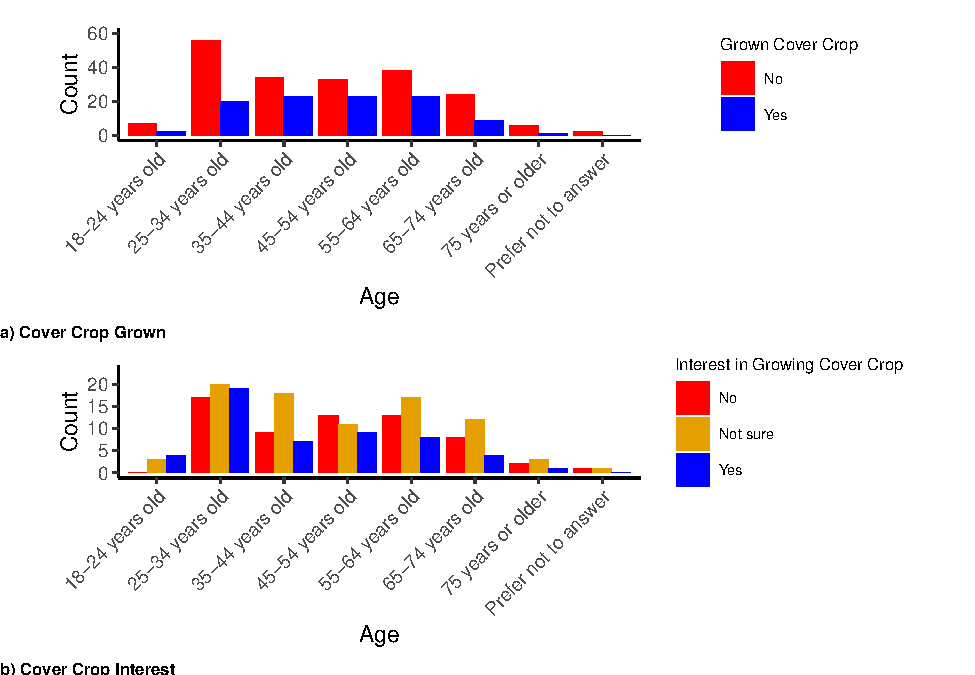
\includegraphics[width=0.9\linewidth]{Project_Template_files/figure-latex/combined age graphs-1} \caption{Respondent's Age by Cover Crop Grown and Cover Crop Interest}\label{fig:combined age graphs}
\end{figure}

\FloatBarrier

I ran a logistic regression to examine the relationship between the age
of the respondents and whether or not they had grown a cover crop in the
last five years. The model showed that the relationship between the two
variables is not significant - age does not affect whether or not a
cover crop was grown (glm; p-value \textgreater{} 0.05). I then ran a
chi-square test of independence to anaylze this relationship further,
and the analysis confirmed that the two variables are independent of one
another (X\^{}2(7, N = 301) = 8.14, p \textgreater{} 0.05).

\begin{Shaded}
\begin{Highlighting}[]
\CommentTok{# Statistical Test 1: GLM}
\NormalTok{Age.Grown.CC <-}\StringTok{ }\KeywordTok{glm}\NormalTok{(Cover.Crop.Grown}\OperatorTok{~}\NormalTok{Age, almonds.CC, }\DataTypeTok{family =}\NormalTok{ binomial)}

\CommentTok{#summary(Age.Grown.CC)}

\KeywordTok{summ}\NormalTok{(Age.Grown.CC)}
\end{Highlighting}
\end{Shaded}

\begin{table}[!h]
\centering
\begin{tabular}{lr}
\toprule
\rowcolor{gray!6}  Observations & 301\\
Dependent variable & Cover.Crop.Grown\\
\rowcolor{gray!6}  Type & Generalized linear model\\
Family & binomial\\
\rowcolor{gray!6}  Link & logit\\
\bottomrule
\end{tabular}
\end{table}

\begin{table}[!h]
\centering
\begin{tabular}{lr}
\toprule
\rowcolor{gray!6}  $\chi^2$(7) & 8.99\\
Pseudo-R² (Cragg-Uhler) & 0.04\\
\rowcolor{gray!6}  Pseudo-R² (McFadden) & 0.02\\
AIC & 391.11\\
\rowcolor{gray!6}  BIC & 420.77\\
\bottomrule
\end{tabular}
\end{table}

\begin{table}[!h]
\centering
\begin{threeparttable}
\begin{tabular}{lrrrr}
\toprule
  & Est. & S.E. & z val. & p\\
\midrule
\rowcolor{gray!6}  (Intercept) & -1.25 & 0.80 & -1.56 & 0.12\\
Age25-34 years old & 0.22 & 0.84 & 0.26 & 0.79\\
\rowcolor{gray!6}  Age35-44 years old & 0.86 & 0.85 & 1.02 & 0.31\\
Age45-54 years old & 0.89 & 0.85 & 1.05 & 0.29\\
\rowcolor{gray!6}  Age55-64 years old & 0.75 & 0.84 & 0.89 & 0.37\\
\addlinespace
Age65-74 years old & 0.27 & 0.89 & 0.30 & 0.76\\
\rowcolor{gray!6}  Age75 years or older & -0.54 & 1.35 & -0.40 & 0.69\\
AgePrefer not to answer & -13.31 & 624.19 & -0.02 & 0.98\\
\bottomrule
\end{tabular}
\begin{tablenotes}
\item Standard errors: MLE
\end{tablenotes}
\end{threeparttable}
\end{table}

\begin{Shaded}
\begin{Highlighting}[]
\CommentTok{# Table 2}

\NormalTok{pretty_Age.GrownCC.glm <-}\StringTok{ }\KeywordTok{prettify}\NormalTok{(}\KeywordTok{summary}\NormalTok{(Age.Grown.CC))}
\end{Highlighting}
\end{Shaded}

\begin{verbatim}
## Waiting for profiling to be done...
\end{verbatim}

\begin{Shaded}
\begin{Highlighting}[]
\KeywordTok{kable}\NormalTok{(pretty_Age.GrownCC.glm,}\DataTypeTok{caption =} \StringTok{"Cover Crop Adoption by Age Ranges of Respondents"}\NormalTok{, }
      \DataTypeTok{align =} \KeywordTok{c}\NormalTok{(}\StringTok{"l"}\NormalTok{, }\KeywordTok{rep}\NormalTok{(}\StringTok{"r"}\NormalTok{, }\DecValTok{3}\NormalTok{)),}\DataTypeTok{format =} \StringTok{"latex"}\NormalTok{, }\DataTypeTok{booktabs =} \OtherTok{TRUE}\NormalTok{)  }\OperatorTok
\StringTok{  }\KeywordTok{kable_styling}\NormalTok{(}\DataTypeTok{latex_options =} \StringTok{"scale_down"}\NormalTok{)}
\end{Highlighting}
\end{Shaded}

\begin{table}

\caption{\label{tab:Question 3}Cover Crop Adoption by Age Ranges of Respondents}
\centering
\resizebox{\linewidth}{!}{
\begin{tabular}[t]{lrrrlrrrl}
\toprule
  & Estimate & Odds Ratio & CI (lower) & CI (upper) & Std. Error & z value & Pr(>|z|) &    \\
\midrule
(Intercept) & -1.2527630 & 0.2857143 & 0.0425711 & 1.182077e+00 & 0.8017837 & -1.5624699 & 0.118 & \\
Age: 25-34 years old & 0.2231436 & 1.2500000 & 0.2742203 & 8.858418e+00 & 0.8430387 & 0.2646896 & 0.791 & \\
Age: 35-44 years old & 0.8618967 & 2.3676471 & 0.5166669 & 1.685549e+01 & 0.8460184 & 1.0187682 & 0.308 & \\
Age: 45-54 years old & 0.8917496 & 2.4393939 & 0.5317246 & 1.737916e+01 & 0.8465450 & 1.0533990 & 0.292 & \\
Age: 55-64 years old & 0.7506710 & 2.1184211 & 0.4641011 & 1.504244e+01 & 0.8441867 & 0.8892239 & 0.374 & \\
\addlinespace
Age: 65-74 years old & 0.2719337 & 1.3125000 & 0.2555195 & 9.922993e+00 & 0.8919837 & 0.3048640 & 0.76 & \\
Age: 75 years or older & -0.5389965 & 0.5833333 & 0.0235138 & 7.681183e+00 & 1.3451854 & -0.4006857 & 0.689 & \\
Age: Prefer not to answer & -13.3133048 & 0.0000017 & NA & 1.388545e+28 & 624.1943416 & -0.0213288 & 0.983 & \\
\bottomrule
\end{tabular}}
\end{table}

\FloatBarrier

\begin{Shaded}
\begin{Highlighting}[]
\CommentTok{# Statistical Test 2: Chi-Square}

\NormalTok{Age.Grown.CC.tbl =}\StringTok{ }\KeywordTok{table}\NormalTok{(almonds.CC}\OperatorTok{$}\NormalTok{Age, almonds.CC}\OperatorTok{$}\NormalTok{Cover.Crop.Grown) }
\NormalTok{Age.Grown.CC.tbl}
\end{Highlighting}
\end{Shaded}

\begin{verbatim}
##                       
##                        No Yes
##   18-24 years old       7   2
##   25-34 years old      56  20
##   35-44 years old      34  23
##   45-54 years old      33  23
##   55-64 years old      38  23
##   65-74 years old      24   9
##   75 years or older     6   1
##   Prefer not to answer  2   0
\end{verbatim}

\begin{Shaded}
\begin{Highlighting}[]
\KeywordTok{chisq.test}\NormalTok{(Age.Grown.CC.tbl)}
\end{Highlighting}
\end{Shaded}

\begin{verbatim}
## 
##  Pearson's Chi-squared test
## 
## data:  Age.Grown.CC.tbl
## X-squared = 8.1357, df = 7, p-value = 0.3208
\end{verbatim}

\FloatBarrier

\subsection{Question 4: How does the size of the respondent's almond
operation affect whether or not they have grown cover crop in the last 5
years?}\label{question-4-how-does-the-size-of-the-respondents-almond-operation-affect-whether-or-not-they-have-grown-cover-crop-in-the-last-5-years}

To assess the effect ``size of operation'' has on cover crop adoption, I
used the numeric responses from the ``total yield-bearing acreage'' text
entry boxes in the survey. I analyzed the responses for ``total
yield-bearing acreage'' rather than ``total non-yield bearing acreage''
because the non-yield bearing trees are not mature enough for
pollination from managed honey bees. Thus, I assumed that non-yield
bearing acreage would be less representative of respondents' behaviors
toward adopting bee-friendly practices.

I then categorized the individual text entries for ``total yield-bearing
acreage'' by ``Small,'' ``Medium,'' and ``Large'' to represent the size
of the operation. The acreage range within each category was determined
by the ALmond Board's almond acre ranges for farm sizes. The ``Small''
category represented producers with 0-40 acres of yield-bearing almonds,
``Medium'' represented producers with 41-200 acres and ``Large''
represented producers with 201+ acres.

To visualize the relationship between the size of the respondent's
almond operation and whether or not they have grown cover crop, I
plotted the two variables. \textbf{Figure 7} shows that ``Small''
operations had the highest frequency of \textbf{not} growing cover crop
in the last five years.

\begin{Shaded}
\begin{Highlighting}[]
\NormalTok{alm.Size =}\StringTok{ }\NormalTok{almonds.CC[almonds.CC}\OperatorTok{$}\NormalTok{Acre.Ranges }\OperatorTok{!=}\StringTok{ " "}\NormalTok{ ,]}
\end{Highlighting}
\end{Shaded}

  \providecommand{\huxb}[2]{\arrayrulecolor[RGB]{#1}\global\arrayrulewidth=#2pt}
  \providecommand{\huxvb}[2]{\color[RGB]{#1}\vrule width #2pt}
  \providecommand{\huxtpad}[1]{\rule{0pt}{\baselineskip+#1}}
  \providecommand{\huxbpad}[1]{\rule[-#1]{0pt}{#1}}

\begin{table}[h]
\begin{raggedright}
\begin{threeparttable}
\begin{tabularx}{0.2\textwidth}{p{0.0666666666666667\textwidth} p{0.0666666666666667\textwidth} p{0.0666666666666667\textwidth}}


\hhline{>{\huxb{0, 0, 0}{0.4}}->{\huxb{0, 0, 0}{0.4}}->{\huxb{0, 0, 0}{0.4}}-}
\arrayrulecolor{black}

\multicolumn{1}{!{\huxvb{0, 0, 0}{0.4}}l!{\huxvb{0, 0, 0}{0}}}{\huxtpad{4pt}\raggedright \textbf{alm.Size.Acre.Ranges}\huxbpad{4pt}} &
\multicolumn{1}{l!{\huxvb{0, 0, 0}{0}}}{\huxtpad{4pt}\raggedright \textbf{alm.Size.Cover.Crop.Grown}\huxbpad{4pt}} &
\multicolumn{1}{r!{\huxvb{0, 0, 0}{0.4}}}{\huxtpad{4pt}\raggedleft \textbf{Freq}\huxbpad{4pt}} \tabularnewline[-0.5pt]


\hhline{>{\huxb{0, 0, 0}{0.4}}->{\huxb{0, 0, 0}{0.4}}->{\huxb{0, 0, 0}{0.4}}-}
\arrayrulecolor{black}

\multicolumn{1}{!{\huxvb{0, 0, 0}{0.4}}l!{\huxvb{0, 0, 0}{0}}}{\cellcolor[RGB]{242, 242, 242}\huxtpad{4pt}\raggedright Large\huxbpad{4pt}} &
\multicolumn{1}{l!{\huxvb{0, 0, 0}{0}}}{\cellcolor[RGB]{242, 242, 242}\huxtpad{4pt}\raggedright No\huxbpad{4pt}} &
\multicolumn{1}{r!{\huxvb{0, 0, 0}{0.4}}}{\cellcolor[RGB]{242, 242, 242}\huxtpad{4pt}\raggedleft 48\huxbpad{4pt}} \tabularnewline[-0.5pt]


\hhline{>{\huxb{0, 0, 0}{0.4}}|>{\huxb{0, 0, 0}{0.4}}|}
\arrayrulecolor{black}

\multicolumn{1}{!{\huxvb{0, 0, 0}{0.4}}l!{\huxvb{0, 0, 0}{0}}}{\huxtpad{4pt}\raggedright Medium\huxbpad{4pt}} &
\multicolumn{1}{l!{\huxvb{0, 0, 0}{0}}}{\huxtpad{4pt}\raggedright No\huxbpad{4pt}} &
\multicolumn{1}{r!{\huxvb{0, 0, 0}{0.4}}}{\huxtpad{4pt}\raggedleft 55\huxbpad{4pt}} \tabularnewline[-0.5pt]


\hhline{>{\huxb{0, 0, 0}{0.4}}|>{\huxb{0, 0, 0}{0.4}}|}
\arrayrulecolor{black}

\multicolumn{1}{!{\huxvb{0, 0, 0}{0.4}}l!{\huxvb{0, 0, 0}{0}}}{\cellcolor[RGB]{242, 242, 242}\huxtpad{4pt}\raggedright Small\huxbpad{4pt}} &
\multicolumn{1}{l!{\huxvb{0, 0, 0}{0}}}{\cellcolor[RGB]{242, 242, 242}\huxtpad{4pt}\raggedright No\huxbpad{4pt}} &
\multicolumn{1}{r!{\huxvb{0, 0, 0}{0.4}}}{\cellcolor[RGB]{242, 242, 242}\huxtpad{4pt}\raggedleft 94\huxbpad{4pt}} \tabularnewline[-0.5pt]


\hhline{>{\huxb{0, 0, 0}{0.4}}|>{\huxb{0, 0, 0}{0.4}}|}
\arrayrulecolor{black}

\multicolumn{1}{!{\huxvb{0, 0, 0}{0.4}}l!{\huxvb{0, 0, 0}{0}}}{\huxtpad{4pt}\raggedright Large\huxbpad{4pt}} &
\multicolumn{1}{l!{\huxvb{0, 0, 0}{0}}}{\huxtpad{4pt}\raggedright Yes\huxbpad{4pt}} &
\multicolumn{1}{r!{\huxvb{0, 0, 0}{0.4}}}{\huxtpad{4pt}\raggedleft 24\huxbpad{4pt}} \tabularnewline[-0.5pt]


\hhline{>{\huxb{0, 0, 0}{0.4}}|>{\huxb{0, 0, 0}{0.4}}|}
\arrayrulecolor{black}

\multicolumn{1}{!{\huxvb{0, 0, 0}{0.4}}l!{\huxvb{0, 0, 0}{0}}}{\cellcolor[RGB]{242, 242, 242}\huxtpad{4pt}\raggedright Medium\huxbpad{4pt}} &
\multicolumn{1}{l!{\huxvb{0, 0, 0}{0}}}{\cellcolor[RGB]{242, 242, 242}\huxtpad{4pt}\raggedright Yes\huxbpad{4pt}} &
\multicolumn{1}{r!{\huxvb{0, 0, 0}{0.4}}}{\cellcolor[RGB]{242, 242, 242}\huxtpad{4pt}\raggedleft 39\huxbpad{4pt}} \tabularnewline[-0.5pt]


\hhline{>{\huxb{0, 0, 0}{0.4}}|>{\huxb{0, 0, 0}{0.4}}|}
\arrayrulecolor{black}

\multicolumn{1}{!{\huxvb{0, 0, 0}{0.4}}l!{\huxvb{0, 0, 0}{0}}}{\huxtpad{4pt}\raggedright Small\huxbpad{4pt}} &
\multicolumn{1}{l!{\huxvb{0, 0, 0}{0}}}{\huxtpad{4pt}\raggedright Yes\huxbpad{4pt}} &
\multicolumn{1}{r!{\huxvb{0, 0, 0}{0.4}}}{\huxtpad{4pt}\raggedleft 37\huxbpad{4pt}} \tabularnewline[-0.5pt]


\hhline{>{\huxb{0, 0, 0}{0.4}}->{\huxb{0, 0, 0}{0.4}}->{\huxb{0, 0, 0}{0.4}}-}
\arrayrulecolor{black}
\end{tabularx}\end{threeparttable}
\par\end{raggedright}

\end{table}\begin{figure}
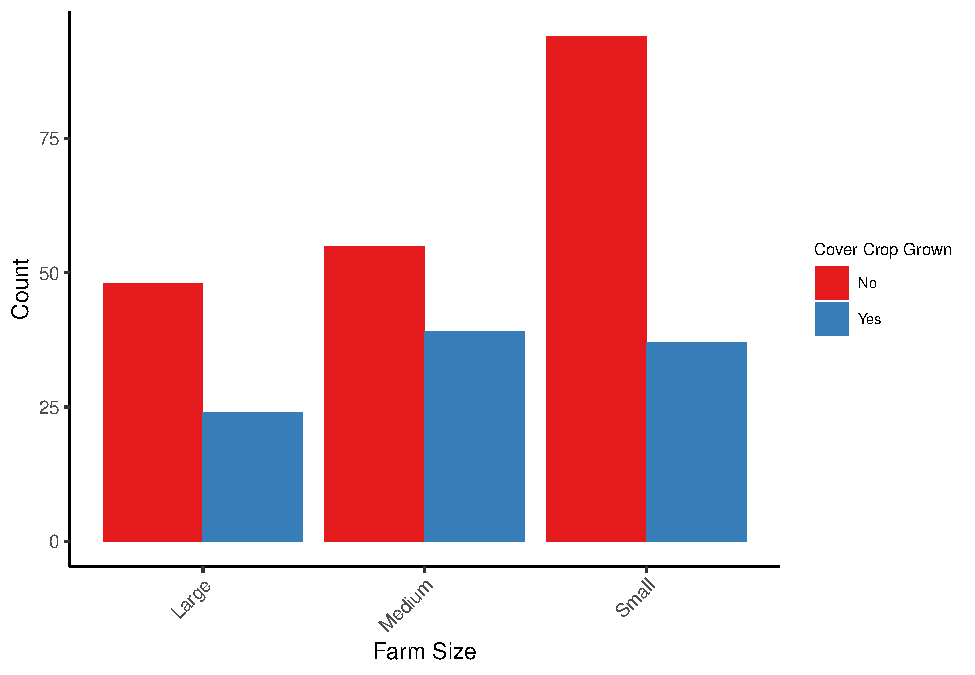
\includegraphics[width=0.9\linewidth]{Project_Template_files/figure-latex/Size plot-1} \caption{Size of Operation by Cover Crop Interest}\label{fig:Size plot}
\end{figure}

\FloatBarrier

Further analysis showed that, unlike the model from \textbf{Question 1}
that controlled for all factors, when solely analyzing cover crop
adoption versus the amount of total yield-bearing acreage, total
yield-bearing acreage does not significantly affect whether the
respondent has grown a cover crop in the last five years (glm; p-value
\textgreater{} 0.05).

\begin{Shaded}
\begin{Highlighting}[]
\NormalTok{Size.GrownCC <-}\StringTok{ }\KeywordTok{glm}\NormalTok{(Cover.Crop.Grown}\OperatorTok{~}\NormalTok{Acre.Ranges , almonds.CC, }\DataTypeTok{family =}\NormalTok{ binomial)}

\CommentTok{#summary(Size.GrownCC)}

\KeywordTok{summ}\NormalTok{(Size.GrownCC)}
\end{Highlighting}
\end{Shaded}

\begin{table}[!h]
\centering
\begin{tabular}{lr}
\toprule
\rowcolor{gray!6}  Observations & 297 (4 missing obs. deleted)\\
Dependent variable & Cover.Crop.Grown\\
\rowcolor{gray!6}  Type & Generalized linear model\\
Family & binomial\\
\rowcolor{gray!6}  Link & logit\\
\bottomrule
\end{tabular}
\end{table}

\begin{table}[!h]
\centering
\begin{tabular}{lr}
\toprule
\rowcolor{gray!6}  $\chi^2$(2) & 4.27\\
Pseudo-R² (Cragg-Uhler) & 0.02\\
\rowcolor{gray!6}  Pseudo-R² (McFadden) & 0.01\\
AIC & 381.19\\
\rowcolor{gray!6}  BIC & 392.27\\
\bottomrule
\end{tabular}
\end{table}

\begin{table}[!h]
\centering
\begin{threeparttable}
\begin{tabular}{lrrrr}
\toprule
  & Est. & S.E. & z val. & p\\
\midrule
\rowcolor{gray!6}  (Intercept) & -0.69 & 0.25 & -2.77 & 0.01\\
Acre.RangesMedium & 0.35 & 0.33 & 1.07 & 0.28\\
\rowcolor{gray!6}  Acre.RangesSmall & -0.24 & 0.32 & -0.76 & 0.45\\
\bottomrule
\end{tabular}
\begin{tablenotes}
\item Standard errors: MLE
\end{tablenotes}
\end{threeparttable}
\end{table}

\begin{Shaded}
\begin{Highlighting}[]
\CommentTok{# Table 3}

\NormalTok{pretty_Size.GrownCC.glm <-}\StringTok{ }\KeywordTok{prettify}\NormalTok{(}\KeywordTok{summary}\NormalTok{(Size.GrownCC))}
\end{Highlighting}
\end{Shaded}

\begin{verbatim}
## Waiting for profiling to be done...
\end{verbatim}

\begin{Shaded}
\begin{Highlighting}[]
\KeywordTok{kable}\NormalTok{(pretty_Size.GrownCC.glm,}\DataTypeTok{caption =} \StringTok{"Cover Crop Adoption by Size of Almond Operation"}\NormalTok{, }
      \DataTypeTok{align =} \KeywordTok{c}\NormalTok{(}\StringTok{"l"}\NormalTok{, }\KeywordTok{rep}\NormalTok{(}\StringTok{"r"}\NormalTok{, }\DecValTok{3}\NormalTok{)),}\DataTypeTok{format =} \StringTok{"latex"}\NormalTok{, }\DataTypeTok{booktabs =} \OtherTok{TRUE}\NormalTok{)  }\OperatorTok
\StringTok{  }\KeywordTok{kable_styling}\NormalTok{(}\DataTypeTok{latex_options =} \StringTok{"scale_down"}\NormalTok{)}
\end{Highlighting}
\end{Shaded}

\begin{table}

\caption{\label{tab:Question 4}Cover Crop Adoption by Size of Almond Operation}
\centering
\resizebox{\linewidth}{!}{
\begin{tabular}[t]{lrrrlrrrl}
\toprule
  & Estimate & Odds Ratio & CI (lower) & CI (upper) & Std. Error & z value & Pr(>|z|) &    \\
\midrule
(Intercept) & -0.6931472 & 0.500000 & 0.3014593 & 0.8073187 & 0.2500000 & -2.7725892 & 0.006 & **\\
Acre.Ranges: Medium & 0.3493756 & 1.418182 & 0.7515922 & 2.7079823 & 0.3260718 & 1.0714684 & 0.284 & \\
Acre.Ranges: Small & -0.2392297 & 0.787234 & 0.4244132 & 1.4733357 & 0.3164889 & -0.7558864 & 0.45 & \\
\bottomrule
\end{tabular}}
\end{table}

\FloatBarrier

\subsection{Question 5: How does the region where the respondent's farm
almonds affect whether or not they have grown cover crop in the last 5
years?}\label{question-5-how-does-the-region-where-the-respondents-farm-almonds-affect-whether-or-not-they-have-grown-cover-crop-in-the-last-5-years}

I performed a chi-square test of independence to examine the
relationship between ``region'' and whether or not respondents have
grown a cover crop in the last five years. The relationship between
these variables is significant, showing that ``region'' does affect
whether or not respondents selected ``Yes'' to having grown a cover crop
(x2(3, N = 301) = 24.205, p \textless{} 0.01). I then ran a logistic
regression to see which regions are most likely to affect whether or not
the respondent has grown a cover crop. The model showed that respondents
with almond acreage located in the San Joaquin and Tulare basins were
significantly less likely to have grown a cover crop in the last five
years than respondents in the Delta region (glm; z = -3.31, p-value
\textless{} 0.05; glm; z = -3.48, p-value \textless{} 0.05).

\begin{Shaded}
\begin{Highlighting}[]
\CommentTok{# Statistical Test 1: Chi-square }
\NormalTok{almonds.CC}\OperatorTok{$}\NormalTok{Regions <-}\StringTok{ }\KeywordTok{as.factor}\NormalTok{(almonds.CC}\OperatorTok{$}\NormalTok{Regions)}

\NormalTok{Region.GrownCC.tbl =}\StringTok{ }\KeywordTok{table}\NormalTok{(almonds.CC}\OperatorTok{$}\NormalTok{Regions, almonds.CC}\OperatorTok{$}\NormalTok{Cover.Crop.Grown) }
\NormalTok{Region.GrownCC.tbl}
\end{Highlighting}
\end{Shaded}

\begin{verbatim}
##                    
##                      No Yes
##   Delta               6  14
##   Sacramento Valley   7  13
##   San Joaquin Basin 125  53
##   Tulare Basin       61  21
\end{verbatim}

\begin{Shaded}
\begin{Highlighting}[]
\KeywordTok{chisq.test}\NormalTok{(Region.GrownCC.tbl)}
\end{Highlighting}
\end{Shaded}

\begin{verbatim}
## 
##  Pearson's Chi-squared test
## 
## data:  Region.GrownCC.tbl
## X-squared = 24.205, df = 3, p-value = 2.263e-05
\end{verbatim}

\begin{Shaded}
\begin{Highlighting}[]
\CommentTok{# Statistical Test 2: GLM}

\NormalTok{Regions.GrownCC.glm <-}\StringTok{ }\KeywordTok{glm}\NormalTok{(Cover.Crop.Grown }\OperatorTok{~}\StringTok{  }\NormalTok{Regions, }
                             \DataTypeTok{data =}\NormalTok{ almonds.CC, }\DataTypeTok{family =}\NormalTok{ binomial )}

\CommentTok{#summary(Regions.GrownCC.glm)}

\KeywordTok{summ}\NormalTok{(Regions.GrownCC.glm)}
\end{Highlighting}
\end{Shaded}

\begin{table}[!h]
\centering
\begin{tabular}{lr}
\toprule
\rowcolor{gray!6}  Observations & 300 (1 missing obs. deleted)\\
Dependent variable & Cover.Crop.Grown\\
\rowcolor{gray!6}  Type & Generalized linear model\\
Family & binomial\\
\rowcolor{gray!6}  Link & logit\\
\bottomrule
\end{tabular}
\end{table}

\begin{table}[!h]
\centering
\begin{tabular}{lr}
\toprule
\rowcolor{gray!6}  $\chi^2$(3) & 22.86\\
Pseudo-R² (Cragg-Uhler) & 0.10\\
\rowcolor{gray!6}  Pseudo-R² (McFadden) & 0.06\\
AIC & 368.42\\
\rowcolor{gray!6}  BIC & 383.24\\
\bottomrule
\end{tabular}
\end{table}

\begin{table}[!h]
\centering
\begin{threeparttable}
\begin{tabular}{lrrrr}
\toprule
  & Est. & S.E. & z val. & p\\
\midrule
\rowcolor{gray!6}  (Intercept) & 0.85 & 0.49 & 1.74 & 0.08\\
RegionsSacramento Valley & -0.23 & 0.68 & -0.34 & 0.74\\
\rowcolor{gray!6}  RegionsSan Joaquin Basin & -1.71 & 0.51 & -3.31 & 0.00\\
RegionsTulare Basin & -1.91 & 0.55 & -3.48 & 0.00\\
\bottomrule
\end{tabular}
\begin{tablenotes}
\item Standard errors: MLE
\end{tablenotes}
\end{threeparttable}
\end{table}

\begin{Shaded}
\begin{Highlighting}[]
\CommentTok{# Table 4}

\NormalTok{pretty_Region.GrownCC <-}\StringTok{ }\KeywordTok{prettify}\NormalTok{(}\KeywordTok{summary}\NormalTok{(Regions.GrownCC.glm))}
\end{Highlighting}
\end{Shaded}

\begin{verbatim}
## Waiting for profiling to be done...
\end{verbatim}

\begin{Shaded}
\begin{Highlighting}[]
\KeywordTok{kable}\NormalTok{(pretty_Region.GrownCC,}\DataTypeTok{caption =} \StringTok{"Cover Crop Adoption by Region"}\NormalTok{, }
      \DataTypeTok{align =} \KeywordTok{c}\NormalTok{(}\StringTok{"l"}\NormalTok{, }\KeywordTok{rep}\NormalTok{(}\StringTok{"r"}\NormalTok{, }\DecValTok{3}\NormalTok{)),}\DataTypeTok{format =} \StringTok{"latex"}\NormalTok{, }\DataTypeTok{booktabs =} \OtherTok{TRUE}\NormalTok{)  }\OperatorTok
\StringTok{  }\KeywordTok{kable_styling}\NormalTok{(}\DataTypeTok{latex_options =} \StringTok{"scale_down"}\NormalTok{)}
\end{Highlighting}
\end{Shaded}

\begin{table}

\caption{\label{tab:Question 5}Cover Crop Adoption by Region}
\centering
\resizebox{\linewidth}{!}{
\begin{tabular}[t]{lrrrlrrrl}
\toprule
  & Estimate & Odds Ratio & CI (lower) & CI (upper) & Std. Error & z value & Pr(>|z|) &    \\
\midrule
(Intercept) & 0.8472979 & 2.3333333 & 0.9360921 & 6.5892453 & 0.4879498 & 1.736445 & 0.082 & .\\
Regions: Sacramento Valley & -0.2282587 & 0.7959184 & 0.2052573 & 3.0138562 & 0.6766648 & -0.337329 & 0.736 & \\
Regions: San Joaquin Basin & -1.7053197 & 0.1817143 & 0.0615139 & 0.4788281 & 0.5147455 & -3.312938 & 0.001 & ***\\
Regions: Tulare Basin & -1.9136493 & 0.1475410 & 0.0469245 & 0.4165938 & 0.5496430 & -3.481622 & <0.001 & ***\\
\bottomrule
\end{tabular}}
\end{table}

\newpage

\section{Summary and Conclusions}\label{summary-and-conclusions}

When controlling for all factors that potentially affect cover crop
adoption, the analyses show that only ``Region'' and ``Total
Yield-Bearing Acreage'' have a significant relationship regarding
whether or not respondents selected ``Yes'' to having grown cover crop
in the last 5 years. However, when the factors are analyzed individually
against ``cover crop adoption,'' the models indicate that only
``Region'' is significant. Upon further analysis, the results also
showed that respondents who farm almonds in the San Joaquin and Tulare
Basins were significantly less likely to select ``Yes'' to having grown
cover crop than respondents in the more northern regions of the
Sacramento Valley and Delta. One explanation for this could be due to
water availability and price. The northern regions in California have a
greater supply of water than those farther south and given the
considerable amount of water used to grow tree crops, it could be that
farmers in the southern regions are more apprehensive about planting
cover crops due to the extra water they necessitate. This being said,
cover crops improve soil health and the soil's water retention
capabilities, so by planting cover crop, the farmers could enhance their
irrigation efficiency.

Cover crop is just one of several bee-friendly practices that almond
producers can adopt on their orchards. However, it is an important
practice as it provides managed honey bees with extra and more diverse
nutrient and pollen sources. By planting a cover crop, producers could
not only improve their soil health but could also strengthen the bee
colonies and obtain better pollination of their almond orchards. As the
demand for almonds continues to increase, more acres of farmland will
transition to almond orchards, and without higher rates of adoption of
bee-friendly practices or a shift in consumer mindset, a continued loss
of managed honey bees in the US appears inevitable. Thus, given the
results from these analyses, industry experts, cost-share programs, and
farm extension agents should work with producers in the southern region
of the state to assist them in funding and educational opportunities
that increase the rates of cover crop adoption.

\newpage

\section{References}\label{references}

\begin{itemize}
\item
  United States Department of Agriculture (USDA). (2019). 2018
  California Almond Acreage Report. California Department of Food and
  Agriculture. Retrieved from
  \url{https://www.nass.usda.gov/Statistics_by_State/California/Publications/Specialty_and_Other_Releases/Almond/Acreage/201904almac.pdf}
\item
  Almond Board of California (ABC). (2019b). Almond Almanac. Almond
  Board of California. Retrieved from
  \url{http://newsroom.almonds.com/sites/default/files/pdf_file/Almanac_2019_Web.pdf}
\end{itemize}

\end{document}
